%% ====================================================================
%%  Supplementary Information
%%  "Energy sovereignty leakage: gas import substitution could relocate
%%   global emissions to mid-century"
%%
%%  Standalone LaTeX (compile separately, or \input into the main file).
%%  Uses the same sn-bibliography.bib. Figure paths point at outputs/figures.
%%  Repo URL + Zenodo DOI filled in (Data and code availability). Confirm
%%  every table value against the final locked-model run before submission.
%% ====================================================================
\documentclass[11pt]{article}
\usepackage[utf8]{inputenc}
\usepackage[T1]{fontenc}
\usepackage{lmodern}
\usepackage[a4paper,margin=1in]{geometry}
\usepackage{graphicx}
\usepackage{float}
\usepackage{booktabs}
\usepackage{amsmath}
\usepackage{longtable}
\usepackage[numbers,sort&compress]{natbib}
\usepackage[hidelinks]{hyperref}
\usepackage[font=small,labelfont=bf]{caption}
\usepackage{xcolor}
\usepackage{listings}
\usepackage{tikz}
\usetikzlibrary{arrows.meta,positioning,shapes.geometric,fit,backgrounds}

% code style for the coupling pseudocode
\lstdefinestyle{coupling}{basicstyle=\ttfamily\footnotesize,
  keywordstyle=\color{blue!60!black}\bfseries, commentstyle=\color{teal!70!black}\itshape,
  numberstyle=\tiny\color{gray}, numbers=left, numbersep=6pt, frame=single,
  framerule=0.3pt, rulecolor=\color{gray!50}, breaklines=true, showstringspaces=false,
  keywords={for,in,if,once,return,def,each,solve,while},
  morecomment=[l]{\#}}

% number SI items as S1, S2, ...
\renewcommand{\thefigure}{S\arabic{figure}}
\renewcommand{\thetable}{S\arabic{table}}
\renewcommand{\theequation}{S\arabic{equation}}
\renewcommand{\thesection}{S\arabic{section}}

% Widen the ToC number boxes so two-digit labels (S10-S12, S11.1) do not
% collide with the section titles.
\makeatletter
\renewcommand*\l@section[2]{%
  \ifnum \c@tocdepth >\z@
    \addpenalty\@secpenalty
    \addvspace{1.0em \@plus\p@}%
    \setlength\@tempdima{2.8em}% was 1.5em
    \begingroup
      \parindent \z@ \rightskip \@pnumwidth
      \parfillskip -\@pnumwidth
      \leavevmode \bfseries
      \advance\leftskip\@tempdima
      \hskip -\leftskip
      #1\nobreak\hfil \nobreak\hb@xt@\@pnumwidth{\hss #2}\par
    \endgroup
  \fi}
\renewcommand*\l@subsection{\@dottedtocline{2}{2.8em}{3.4em}}
\makeatother

\title{\textbf{Supplementary Information}\\[4pt]
Energy sovereignty leakage: gas import substitution could relocate global
emissions to mid-century}
\author{}
\date{}

\begin{document}
\maketitle
\tableofcontents
\vspace{1em}

\noindent This Supplementary Information is organised in two parts.
\textbf{Part~I --- Model details} (Sections~\ref{si:regions}--\ref{si:coupling-fwd})
documents the regions and their country composition, the supply curves and
convex reformulation, the locked parameters, and the PyPSA\,$\times$\,Brightway
emissions coupling. \textbf{Part~II --- Data, validation and results}
(Sections~\ref{si:market}--\ref{si:emissions}) presents the descriptive market
context benchmarked against the Global Gas Report~2025 \citep{ggr2025}, the
out-of-sample back-cast, and the full set of threshold, scenario, uncertainty,
regional and emissions results referenced in the main text.

\begin{center}\rule{0.6\linewidth}{0.4pt}\\[2pt]
\textsc{Part~I\quad Model details}\\
\rule{0.6\linewidth}{0.4pt}\end{center}

% ---------------------------------------------------------------
\section{Model regions and network}\label{si:regions}

The model represents global gas trade over 19 market regions
(Table~\ref{tab:regions}). Each region carries one or more production
generators disaggregated by resource type, a demand load, and, where
relevant, a coal-to-gas switchable demand tranche. Regions are connected by
capacitated transport links representing pipelines and LNG corridors. A
high-cost slack generator at every node guarantees feasibility and is
verified to remain unused in all solved years.

\begin{longtable}{@{}lll@{}}
\caption{The 19 model regions, their principal domestic supply type, and
their role in the gas trade. Study-focus regions in bold.}\label{tab:regions}\\
\toprule
\textbf{Region} & \textbf{Principal supply} & \textbf{Trade role} \\
\midrule
\endfirsthead
\toprule
\textbf{Region} & \textbf{Principal supply} & \textbf{Trade role} \\
\midrule
\endhead
\textbf{USA}            & Shale (Gulf, Permian, Appalachia) & Producer / LNG exporter \\
\textbf{Mexico}         & Conventional + (nascent) shale    & Importer / sovereignty case \\
Canada                  & Conventional / shale              & Producer / LNG exporter \\
Europe                  & Norwegian offshore + imports      & Importer \\
China                   & Domestic + imports                & Importer (coal-switch) \\
South Asia              & Domestic + imports                & Importer (coal-switch) \\
Southeast Asia          & Domestic + imports                & Importer (coal-switch) \\
Northeast Asia          & Imports                           & Importer (coal-switch) \\
Latin America           & Argentine shale + imports         & Mixed \\
Russia                  & Conventional                      & Producer / exporter \\
Iran                    & Conventional                      & Producer \\
Gulf States             & Conventional                      & Producer / exporter \\
Qatar                   & LNG                               & LNG exporter \\
North Africa            & Conventional                      & Producer / exporter \\
Sub-Saharan Africa      & LNG                               & LNG exporter \\
Central Asia            & Conventional                      & Exporter (pipeline to China) \\
Caspian region          & Conventional                      & Exporter \\
Australia               & LNG                               & LNG exporter \\
US-LNG (hub)            & ---                               & Liquefaction/export node \\
\bottomrule
\end{longtable}

Each model region aggregates the countries and territories in
Table~\ref{tab:composition}; regional gas demand is the sum of member-country
demand, and the country-to-region map is the one used to fill national polygons
in the resource map (main text, Fig.~1) and to attribute per-region emissions
in the coupling (Section~\ref{si:coupling}).

\begin{longtable}{@{}lp{0.68\linewidth}@{}}
\caption{Composition of the model regions: constituent countries and
territories. Single-country regions (USA, Canada, Mexico, Russia, China, Iran,
Qatar) are modelled at national resolution; the US-LNG hub is a liquefaction
node, not a country.}\label{tab:composition}\\
\toprule
\textbf{Region} & \textbf{Constituent countries / territories} \\
\midrule
\endfirsthead
\toprule
\textbf{Region} & \textbf{Constituent countries / territories} \\
\midrule
\endhead
\textbf{USA}        & United States \\
\textbf{Mexico}     & Mexico \\
Canada             & Canada \\
Europe             & EU-27 (incl.\ Germany, France, Italy, Spain, Netherlands, Poland), United Kingdom, Norway, Switzerland, Ukraine, Western Balkans, Belarus, Moldova \\
Russia             & Russia \\
China              & China \\
South Asia         & India, Pakistan, Bangladesh, Sri Lanka, Nepal, Bhutan, Maldives \\
Southeast Asia     & Indonesia, Malaysia, Thailand, Vietnam, Singapore, Philippines, Myanmar, Brunei, Cambodia, Laos, Timor-Leste \\
Northeast Asia     & Japan, South Korea, Taiwan, Mongolia, North Korea \\
Latin America      & Brazil, Argentina, Chile, Bolivia, Peru, Colombia, Venezuela, Ecuador, and Central America \& Caribbean states (incl.\ Trinidad and Tobago) \\
North Africa       & Algeria, Egypt, Libya, Morocco, Tunisia \\
Sub-Saharan Africa & Nigeria, Mozambique, Angola, Tanzania, Senegal and other producers \\
Iran               & Iran \\
Gulf States        & Saudi Arabia, United Arab Emirates, Kuwait, Oman, Bahrain \\
Qatar              & Qatar \\
Central Asia       & Turkmenistan, Uzbekistan, Kazakhstan, Kyrgyzstan, Tajikistan \\
Caspian region     & Azerbaijan, Georgia, Armenia \\
Australia          & Australia, New Zealand, Papua New Guinea \\
US-LNG (hub)       & --- (liquefaction/export node) \\
\bottomrule
\end{longtable}

% ---------------------------------------------------------------
\section{Supply curves and convex reformulation}\label{si:curves}

Three margins that govern leakage are represented as rising marginal-cost
curves rather than single cost blocks (main text, Methods).

\paragraph{US production.} A depletion-style step curve by resource type
(\texttt{data/us\_supply\_curve.csv}). Tranche~0 approximates current
production at Henry-Hub cost; higher tranches add incremental
technically-recoverable resource at rising breakeven, so the marginal cost of
the next US molecule increases with cumulative output. The rising curve also
embodies the supply-side logic that costlier, higher-breakeven resource is the
first to remain unextracted when demand falls short
\citep{Welsby2021, GreenDenniss2018}.

\paragraph{US liquefaction.} A rising-cost curve of tolling tranches
(model \$/MMBtu-equivalent, $\sim$2.0--5.0) whose cumulative capacity grows
over time. In 2025 only existing brownfield capacity ($\sim$150~BCM) is
exposed, keeping the baseline realistic; later expansion costs progressively
more. This replaces a single endogenous liquefaction link and makes the
export response smooth rather than an on/off capacity wall.

\paragraph{Coal-to-gas switching.} A spread of coal-parity prices
representing a heterogeneous coal fleet, rather than one threshold
(\texttt{COAL\_PARITY\_SPREAD}, 13 steps over $\pm$2.0 around the central
parity of 6.5). The spread reflects the real dispersion in the
delivered-gas price at which individual coal units switch, given differences
in efficiency, flexibility and location \citep{GonzalezSalazar2018}; the
consequences of rapid, price-driven coal-to-gas substitution have been analysed
in detail for the Chinese power sector \citep{Qin2017}.

\paragraph{Price-elastic demand.} Regional demand responds to the delivered
price around a reference point (\texttt{DEMAND\_REF\_PRICE}), with a modest
elasticity in the range reported by meta-analyses of energy demand
\citep{Labandeira2017}; this is the channel through which costlier Mexican
shale curtails part of domestic gas use.

\paragraph{Convexity.} To remove the corner solutions of a pure linear
program---under which the leaked volume can jump discontinuously between
markets---a small per-generator quadratic cost term is added
(\texttt{QUADRATIC\_SLOPE}~$=0.8$~\$/MMBtu across a generator's full
capacity). The objective becomes strictly convex and the optimum unique. This
follows recommended practice for transparent, reproducible energy-system
optimisation \citep{DeCarolis2017}. Supplementary
Table~\ref{tab:params} lists the governing parameters.

\begin{table}[H]\centering
\caption{Central model parameters (locked). See \texttt{src/config.py}.}\label{tab:params}
\begin{tabular}{@{}lll@{}}
\toprule
Parameter & Symbol / key & Central value \\
\midrule
Gas combustion CO\textsubscript{2}       & $E_{\mathrm{comb}}$      & 56 gCO\textsubscript{2}/MJ \\
US shale methane-leakage rate            & $r_{\mathrm{CH4}}$       & 2.5\% (range 1.5--3.7) \\
CH\textsubscript{4} GWP (100~yr / 20~yr) & $\mathrm{GWP_{CH4}}$     & 30 / 82.5 \\
LNG lifecycle penalty                    & $\lambda_{\mathrm{LNG}}$ & 0.25 \\
Coal lifecycle intensity (100/20)        & $I_{\mathrm{coal}}$      & 108 / 126 \\
Coal-parity (central)                    & \texttt{COAL\_PARITY}    & 6.5 \$/MMBtu \\
Reliability premium (central)            & $\rho$                   & 1.0 \$/MMBtu (0--2.5) \\
Carbon price sweep                       & $\tau$                   & \$0--42/tCO\textsubscript{2} \\
Quadratic convexity slope                & \texttt{QUADRATIC\_SLOPE}& 0.8 \$/MMBtu \\
US export-capacity axis                  & \texttt{us\_supply\_scale}& 0.7--1.3 (central 1.0) \\
\bottomrule
\end{tabular}
\end{table}

% ---------------------------------------------------------------
\section{Emissions coupling framework (overview)}\label{si:coupling-fwd}

Emissions are not applied as fixed factors but computed by coupling the trade
optimisation to a process-lifecycle inventory: lifecycle greenhouse-gas
intensities are evaluated once in Brightway \citep{Mutel2017, Steubing2020} on
the ecoinvent~3.9.1 background database \citep{Wernet2016} under an IPCC~2021
characterisation \citep{ipcc_ar6_wg1} and, because impact scores are linear in the functional unit,
applied to each solved year's dispatch to yield per-region, per-year emissions
at both GWP horizons. This is the modelling contribution that turns a
least-cost gas-trade model into a lifecycle-consistent one. The full procedure
---the intensity equation $I_{\mathrm{gas}}=a+b\,r$, the per-region ledger, the
methodology flowchart (Extended Data Fig.~1) and the coupling pseudocode
(Listing~\ref{lst:coupling})---is given in Section~\ref{si:coupling}; the
intensities themselves and their stage decomposition are in
Section~\ref{si:emissions}.

\begin{center}\rule{0.6\linewidth}{0.4pt}\\[2pt]
\textsc{Part~II\quad Data, validation and results}\\
\rule{0.6\linewidth}{0.4pt}\end{center}

% ---------------------------------------------------------------
\section{Market context benchmarked against the Global Gas Report}\label{si:market}

Before the model-specific results, we place the solved system against the
observed 2024--25 gas market as reported in the Global Gas Report~2025
\citep{ggr2025}. These panels are drawn entirely from this study's inputs and
solved outputs; the report is used only as an external yardstick.

\paragraph{Regional demand.} Modelled gas demand diverges across regions over
2025--2045 (Fig.~\ref{fig:ggr-demand}): Asian demand---led by China---rises
steeply while European demand declines, the same structural pattern the report
documents for the observed market. This is the demand backdrop against which US
gas competes for the marginal Asian buyer.

\begin{figure}[H]\centering
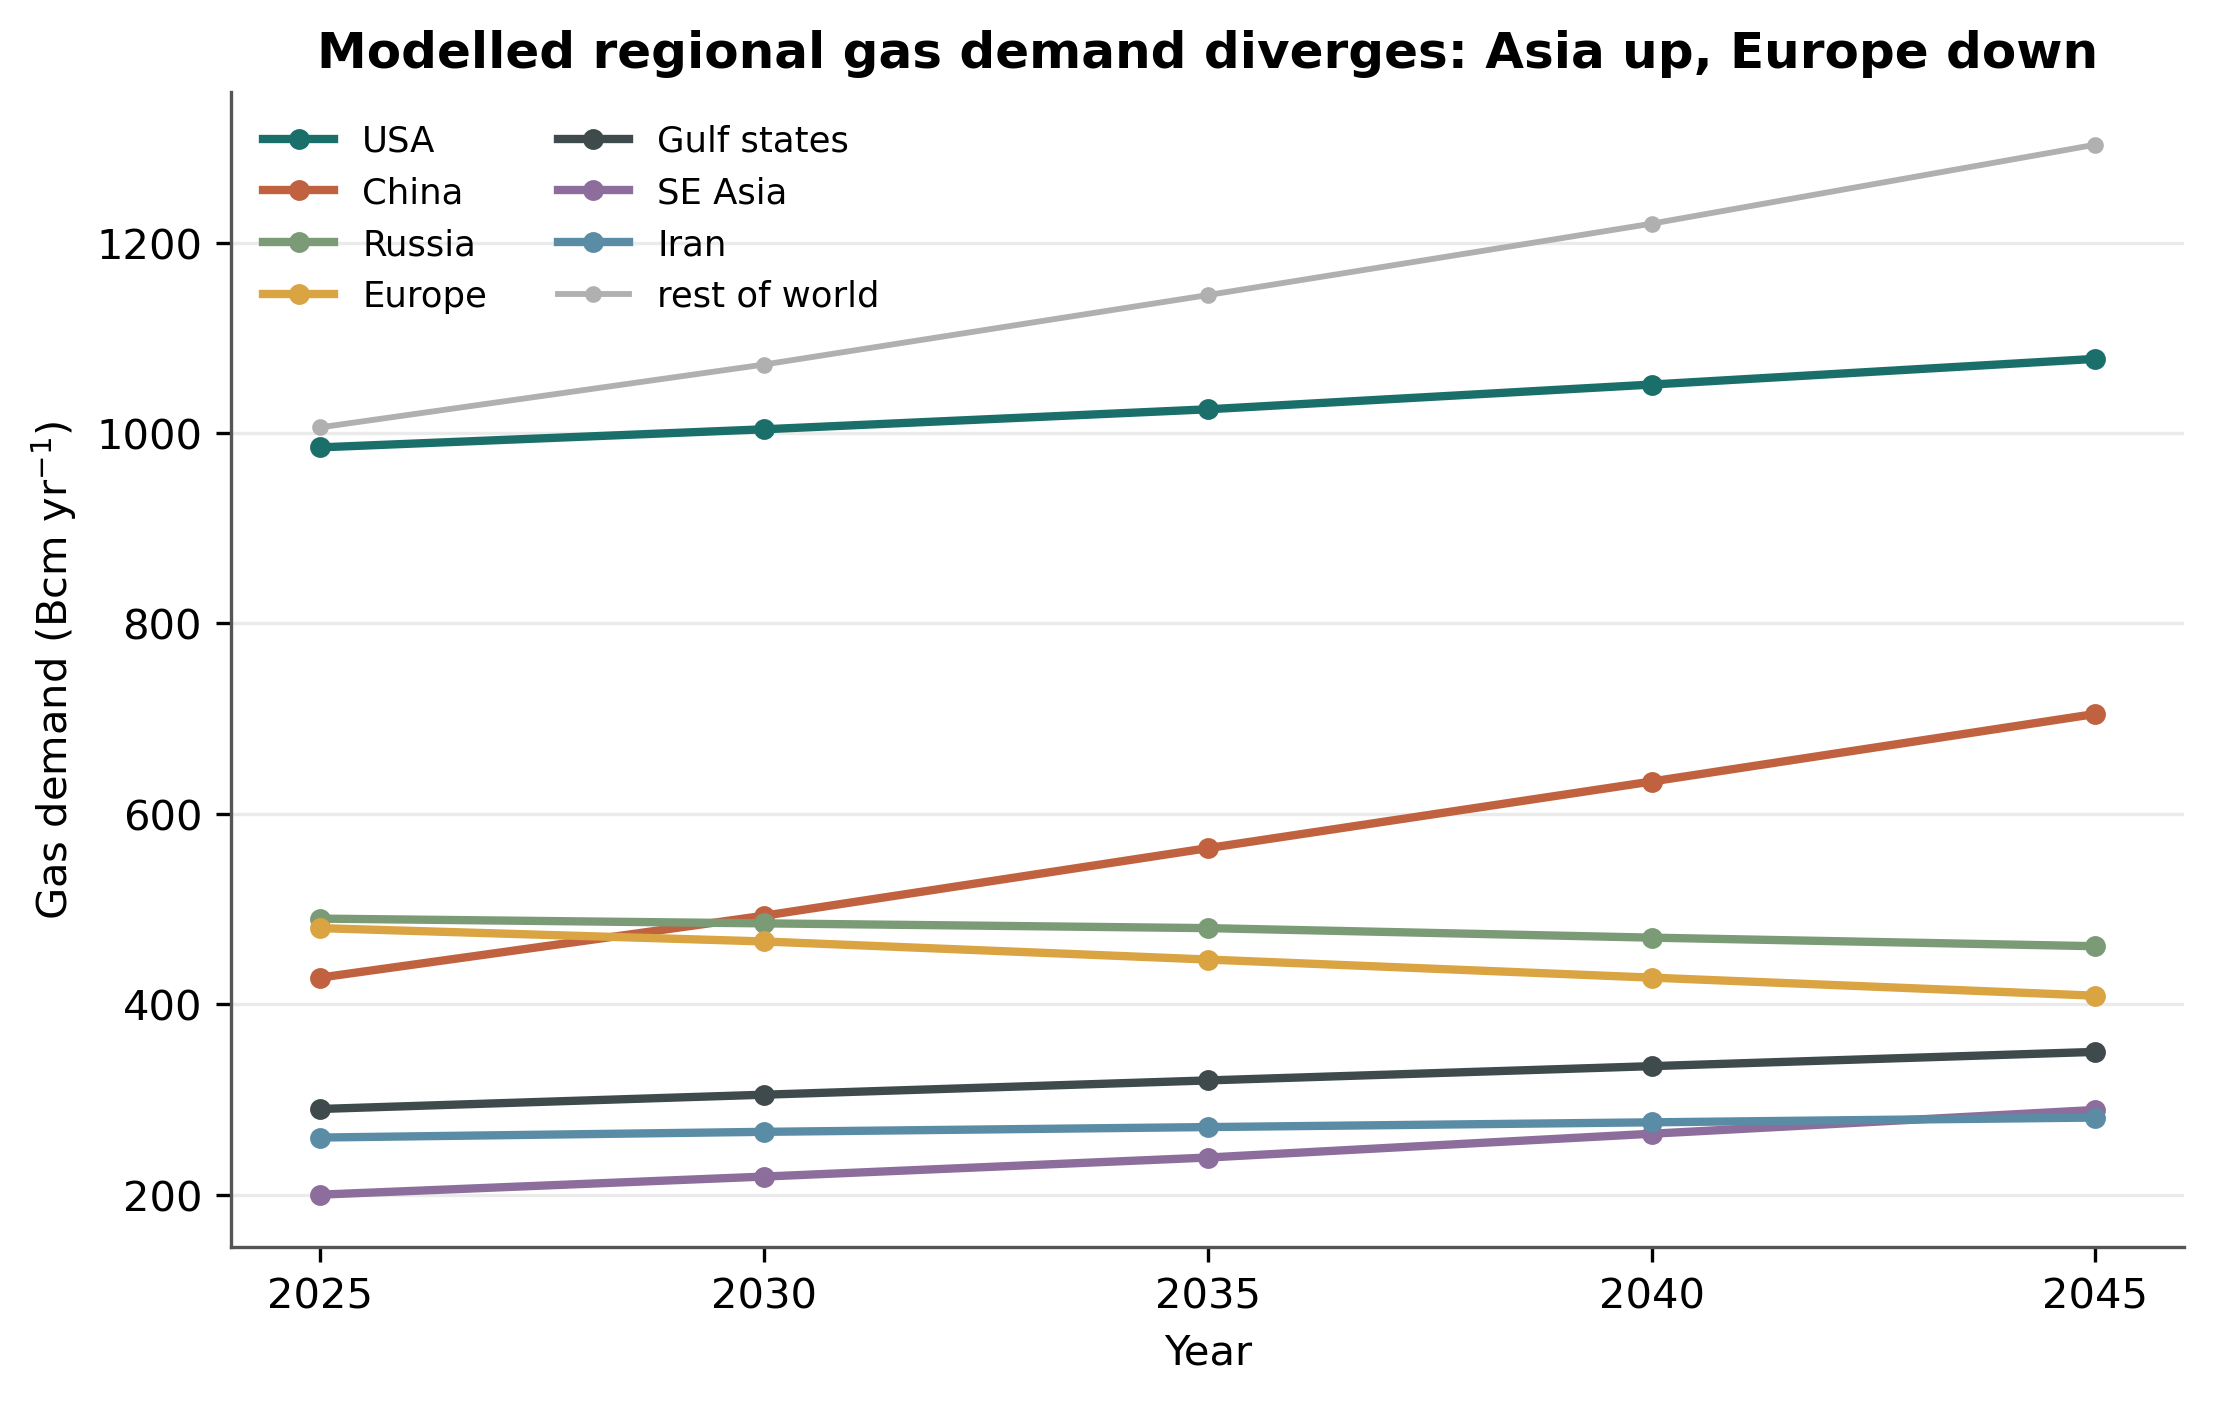
\includegraphics[width=0.82\linewidth]{outputs/figures/GGR_G2_regional_demand.png}
\caption{Modelled regional gas demand, 2025--2045 (BCM per year). The seven
largest 2045 markets are shown individually; remaining regions are aggregated.
China overtakes as the principal growth market while Europe contracts,
consistent with the demand trajectories in the Global Gas Report~2025
\citep{ggr2025}.}\label{fig:ggr-demand}
\end{figure}

\paragraph{Net trade balance.} The solved 2025 net-trade ranking
(Fig.~\ref{fig:ggr-trade}) reproduces the observed structure of the global gas
market: the United States, Russia, Qatar, Australia and the Gulf as the leading
net exporters, and Europe, China and Northeast Asia as the largest net
importers. Mexico appears as a major net importer at $\sim$64~BCM, closely
matching its observed 68~BCM and fourth-place global ranking \citep{ggr2025};
this correspondence is the empirical anchor for treating Mexico as the
sovereignty test case. China's modelled net import is larger than the reported
figure because the model routes its coal-to-gas switchable demand through gas,
an intentional feature of the leakage experiment rather than a demand forecast
(Section~\ref{si:validation}).

\begin{figure}[H]\centering
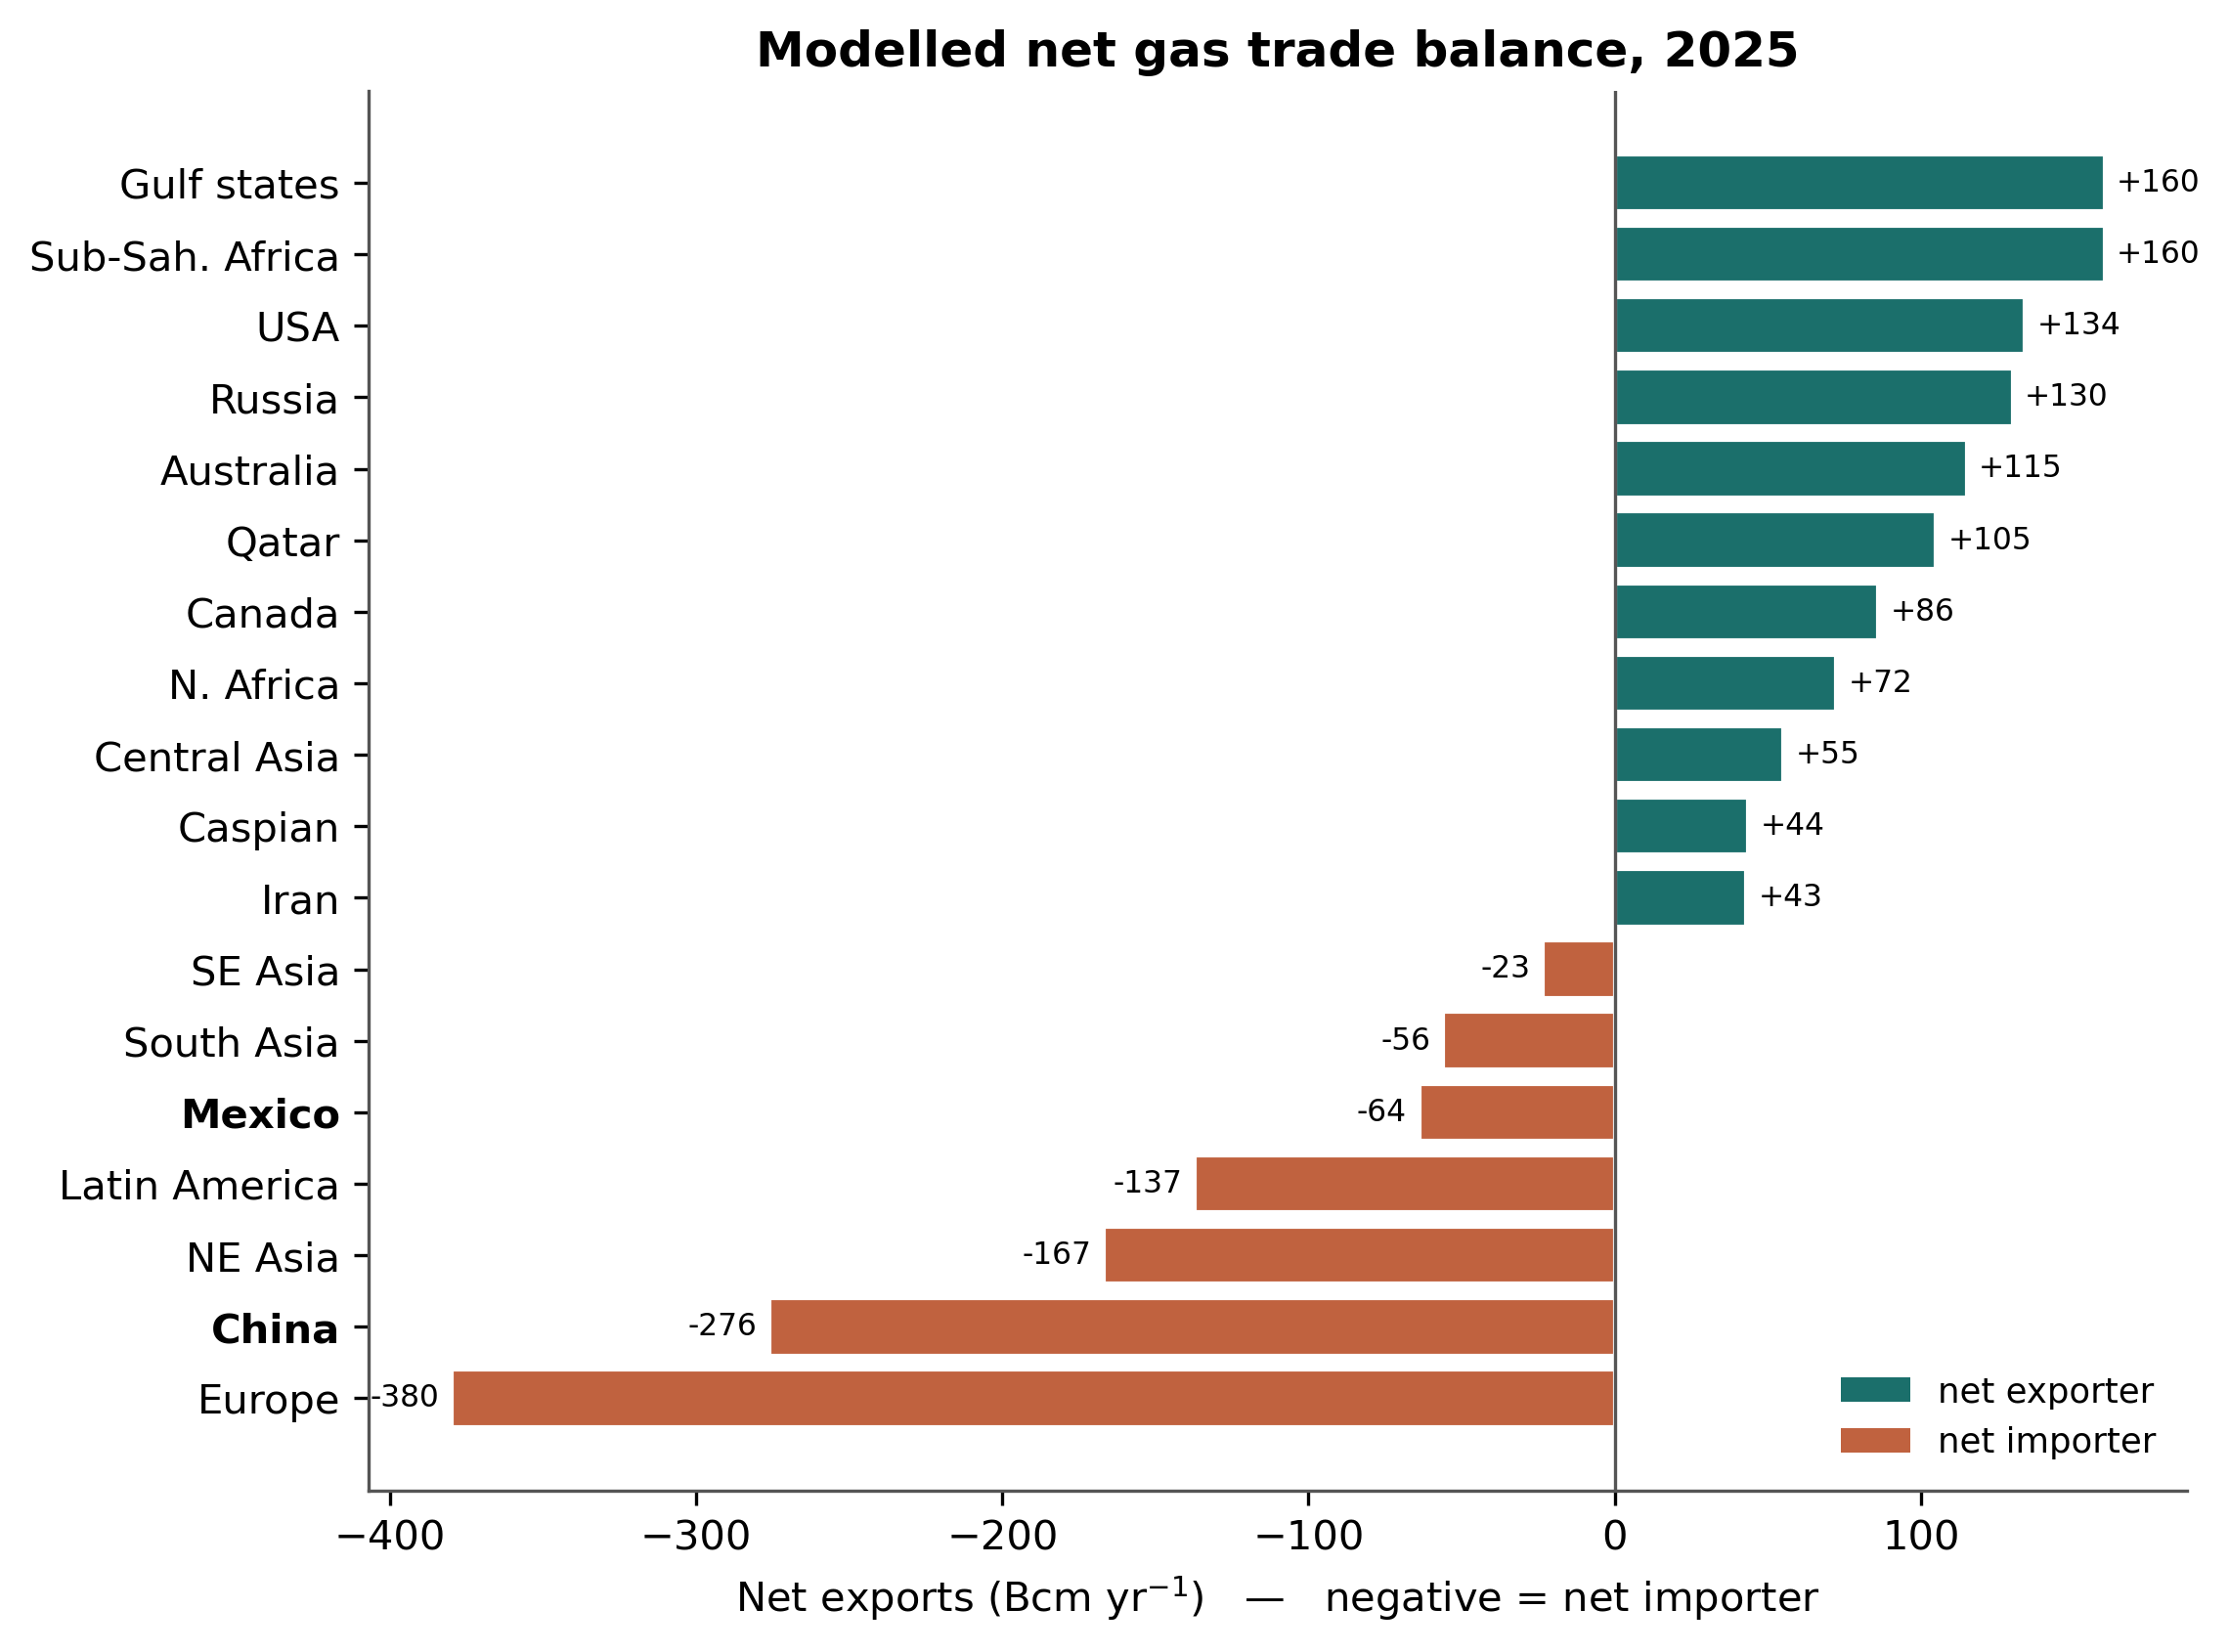
\includegraphics[width=0.8\linewidth]{outputs/figures/GGR_G3_net_trade_ranking.png}
\caption{Modelled net gas trade balance by region, 2025 (BCM per year;
positive~=~net exporter). Mexico and China are highlighted. The exporter/
importer structure matches the Global Gas Report~2025 top-8 rankings; Mexico's
modelled $\sim$64~BCM net import tracks the observed 68~BCM
\citep{ggr2025}.}\label{fig:ggr-trade}
\end{figure}

\paragraph{The export-arbitrage margin.} The US step supply curve
(Fig.~\ref{fig:ggr-supply}) sets how much US gas can reach Asia below the
coal-parity wall---the headroom that the \texttt{us\_supply\_scale} axis sweeps.
Only the low-cost tranches clear the wall once the LNG chain is added; the
high-cost tranches form the price ceiling that keeps leakage near zero under
present-day prices. This is the supply-side counterpart to the delivered-to-Asia
merit-order figure in the main text.

\begin{figure}[H]\centering
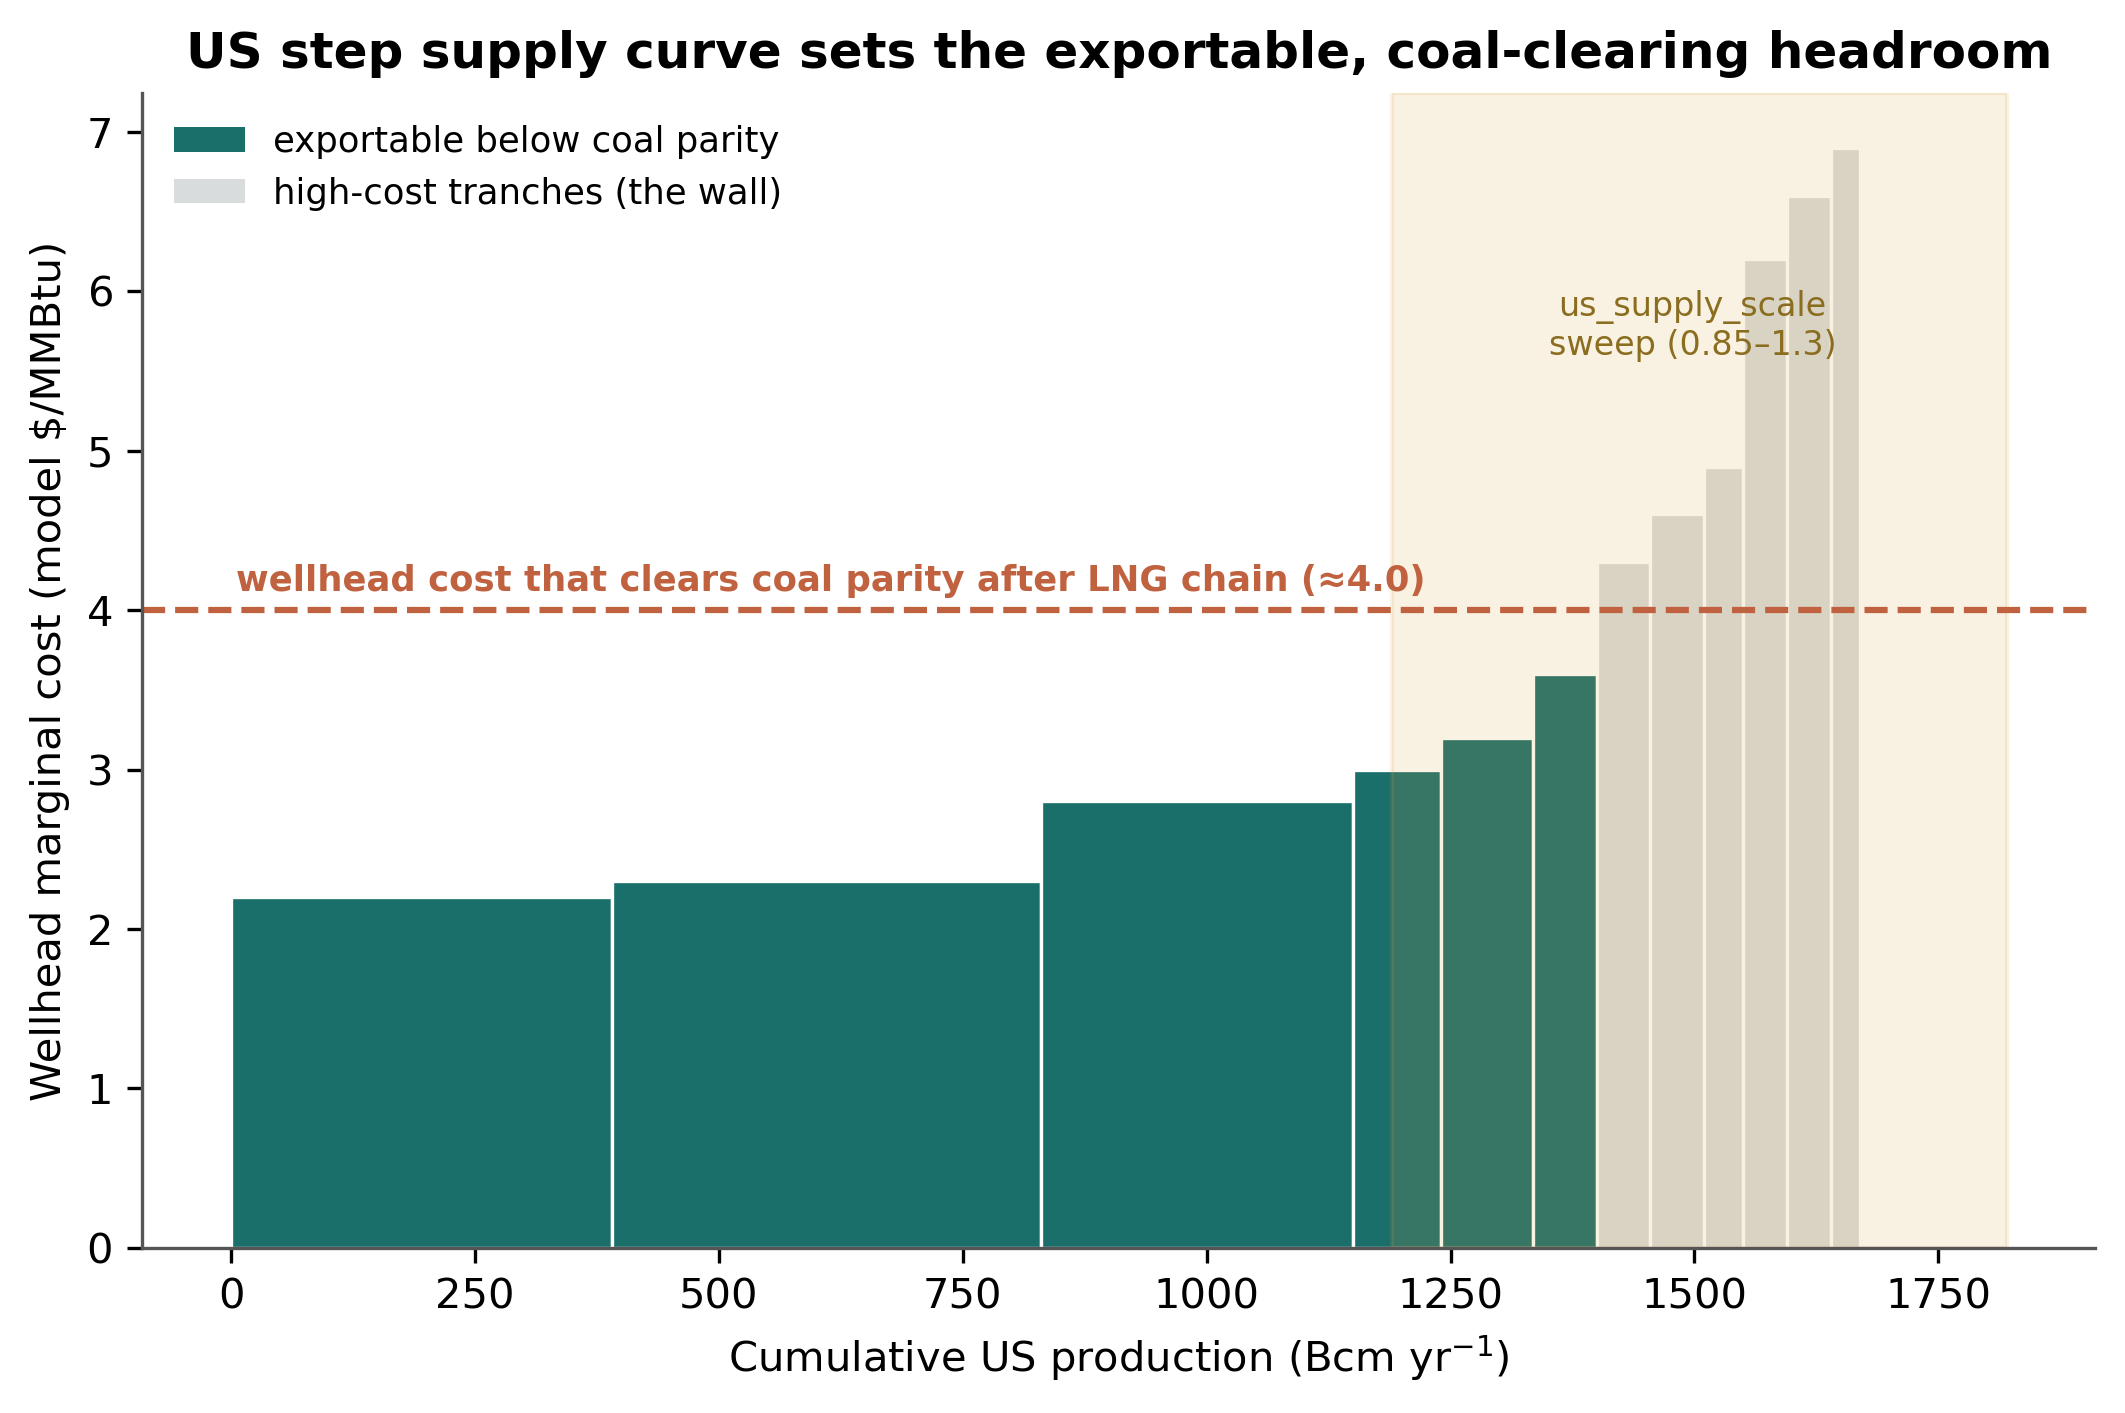
\includegraphics[width=0.82\linewidth]{outputs/figures/GGR_G4_us_supply_curve.png}
\caption{US wellhead step supply curve (BCM per year). Tranches below the
dashed line clear the coal-parity price once liquefaction, capital and shipping
are added and are therefore exportable into the coal-to-gas channel; the gold
band shows the \texttt{us\_supply\_scale} sweep (0.85--1.3) that defines the
conditional leakage range.}\label{fig:ggr-supply}
\end{figure}

% ---------------------------------------------------------------
\section{Out-of-sample validation (back-cast)}\label{si:validation}

The model is calibrated to 2025 only. To test it out of sample we drive it
with historical regional demand for 2018, 2021 and 2023---years it was not
tuned to---and compare modelled trade with observed figures
(Table~\ref{tab:validation}; \texttt{src/validation.py};
\texttt{data/validation\_history.csv}), drawn from
statistical energy reviews and agency outlooks \citep{EI2024, iea_weo2024} and,
for the emissions cross-checks, from standardised historical inventories
\citep{Hoesly2018}. For the
back-cast the forward-looking constructs (coal-to-gas switching demand,
elastic-demand substitution) are disabled and US liquefaction is capped at
the historically observed export level, so importer flows and US LNG are not
inflated by future infrastructure.

\begin{table}[H]\centering
\caption{Out-of-sample back-cast: modelled versus observed trade
(BCM~yr\textsuperscript{-1}), 2018--2023. The model was calibrated to 2025
only.}\label{tab:validation}
\begin{tabular}{@{}llrrr@{}}
\toprule
Year & Metric & Observed & Modelled & Error (\%) \\
\midrule
2018 & US production        & 840  & 929  & $+11$ \\
2018 & US LNG exports       & 28   & 28   & $0$ \\
2018 & Norway exports       & 120  & 125  & $+4$ \\
2018 & US$\to$Mexico pipe   & 50   & 89   & $+78$ \\
2021 & US production        & 934  & 983  & $+5$ \\
2021 & Norway exports       & 113  & 125  & $+11$ \\
2023 & US production        & 1035 & 1066 & $+3$ \\
2023 & Norway exports       & 110  & 125  & $+14$ \\
\bottomrule
\end{tabular}
\end{table}

The core North Atlantic supply quantities that the paper turns on are
reproduced well out of sample (Supplementary Fig.~\ref{fig:validation}): US
marketed production is within 3--11\% across all three back-cast years, and
Norwegian exports within 4--14\%; US LNG exports are matched by construction
(capped at the observed level, since liquefaction capacity is a known historical
constraint). The
US$\to$Mexico pipeline is matched only approximately and we treat it as stylised:
it is over-predicted because the model routes cheap US gas to Mexico more
aggressively than the historical contract- and infrastructure-limited flow.
Chinese imports are deliberately excluded from the quantitative back-cast: at the
single-region aggregation used, the one ``China'' node cannot represent the
pipeline-versus-LNG and domestic-supply structure that shaped historical Chinese
imports, and modelled imports over-predict the observed level by roughly a factor
of four---so we treat China's import \emph{level} as stylised and do not read it
quantitatively. Neither limitation affects the ESL mechanism, which depends on
the delivered-US-LNG-versus-Asian-coal margin rather than on reproducing Chinese
import levels; both bound the resolution at which regional import totals should
be read.

\begin{figure}[H]\centering
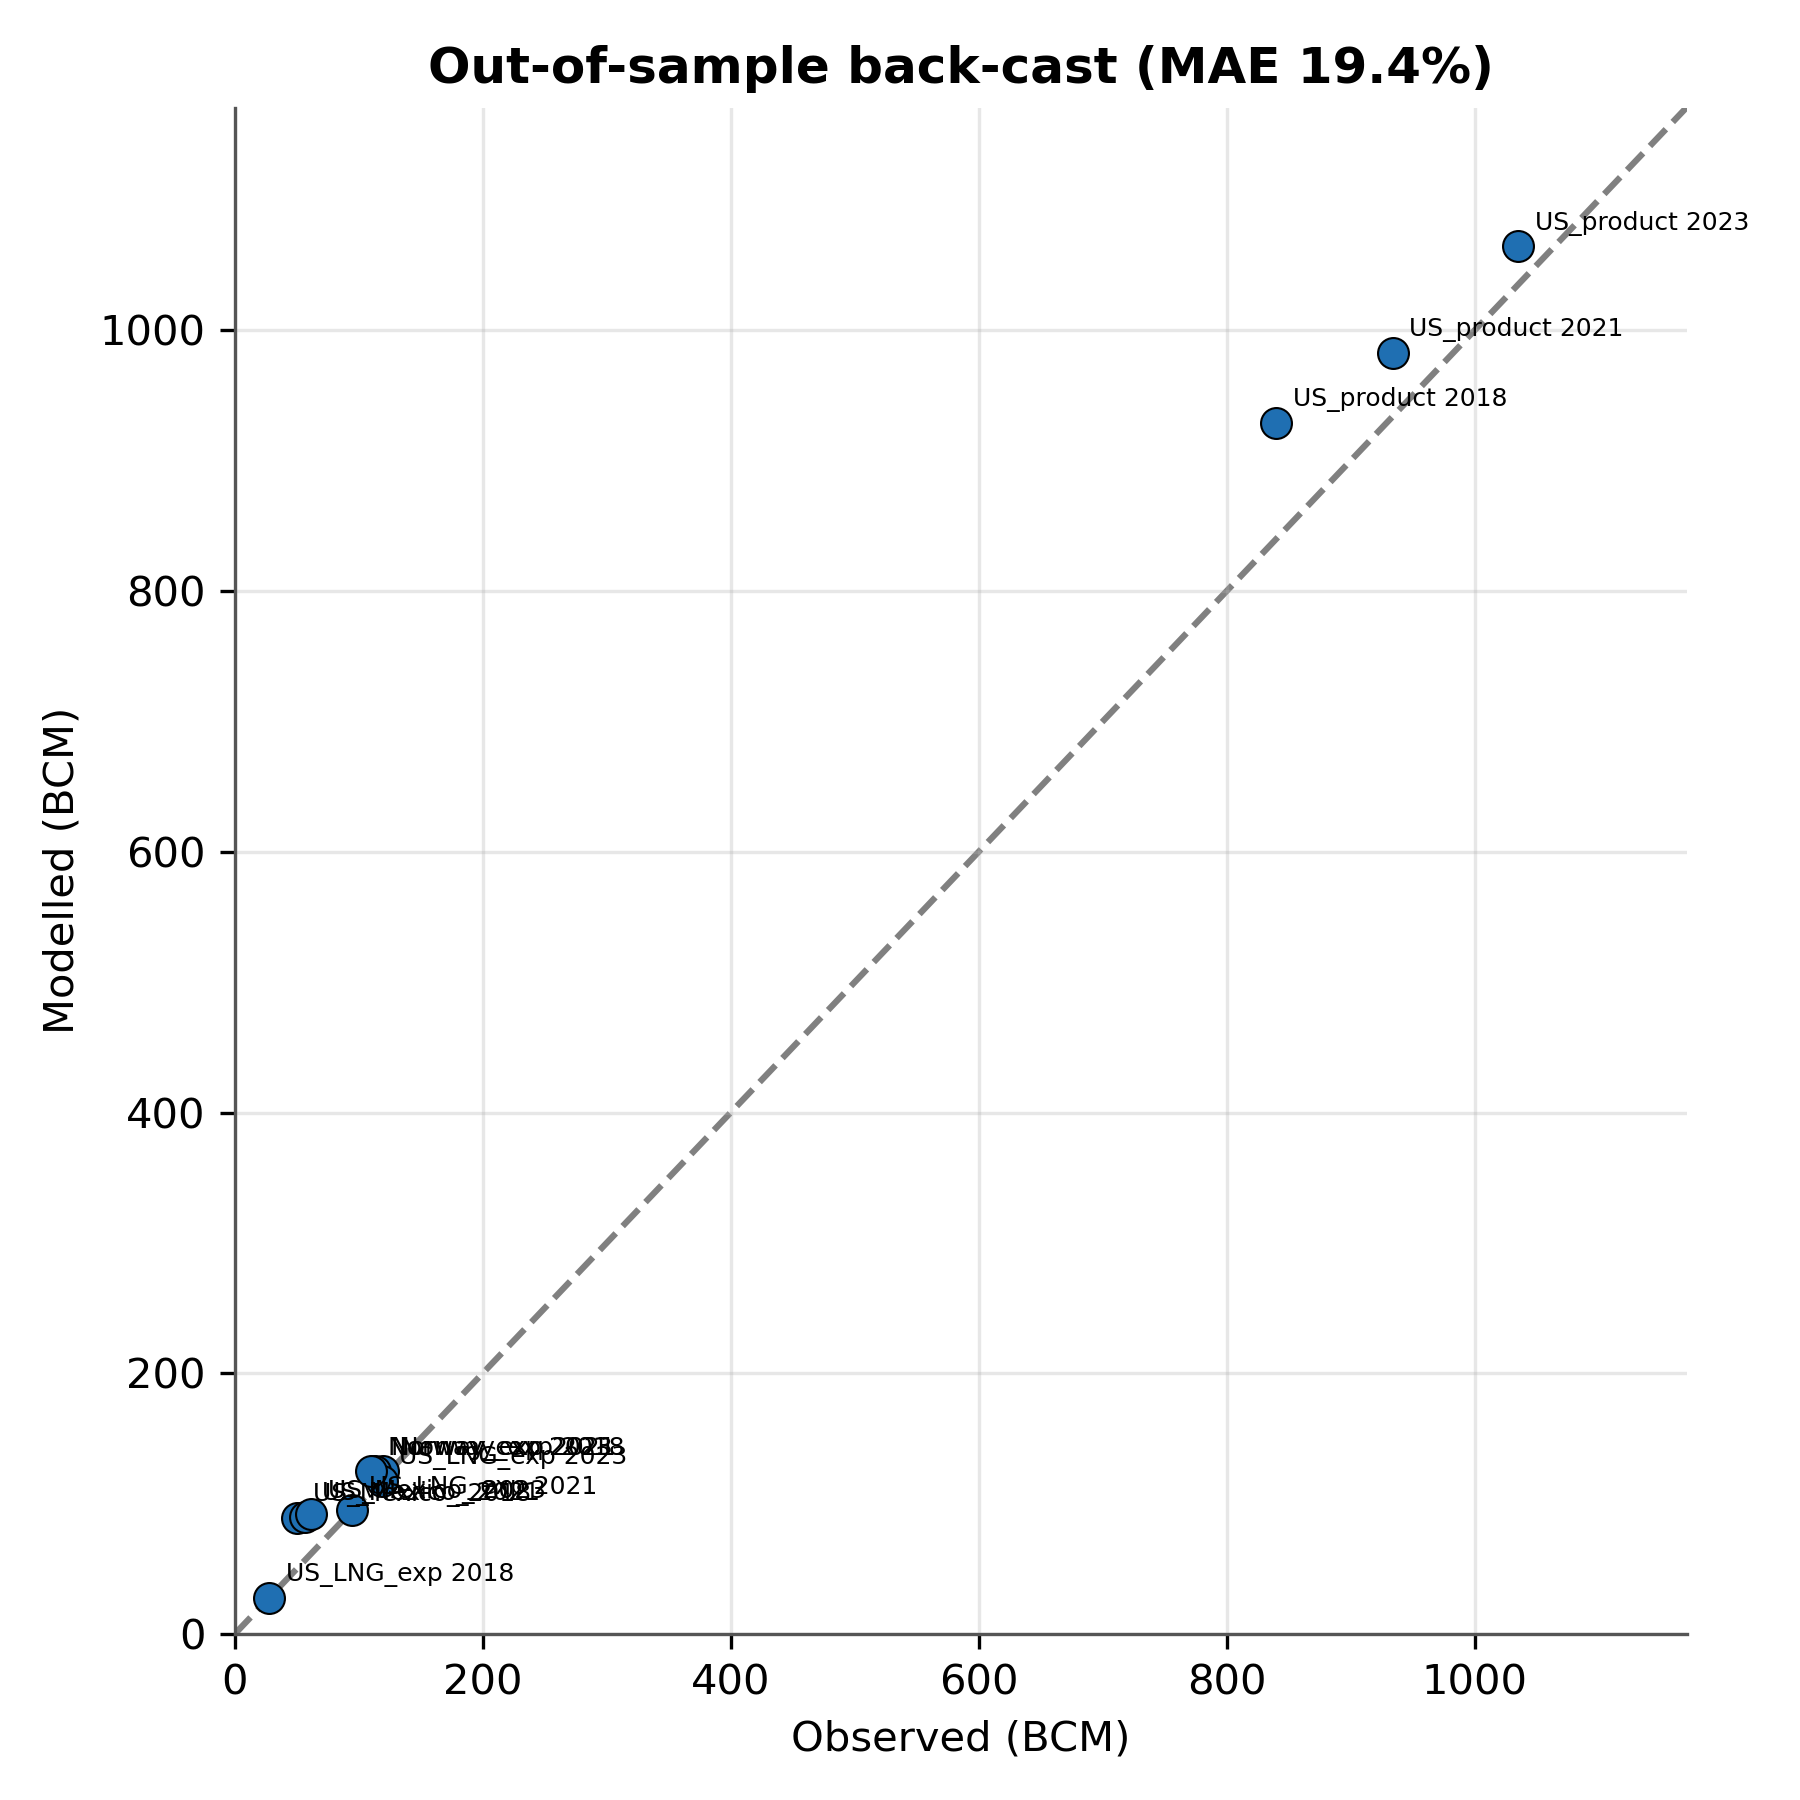
\includegraphics[width=0.6\linewidth]{outputs/figures/Validation_backcast.png}
\caption{Out-of-sample back-cast: modelled versus observed inter-regional
trade for 2018--2023. Points on the 1:1 line indicate agreement; the mean
absolute error is reported in the panel title.}\label{fig:validation}
\end{figure}

% ---------------------------------------------------------------
\section{Threshold behaviour: reliability premium and carbon price}\label{si:threshold}

Energy Sovereignty Leakage switches on only once delivered US LNG into Asia
falls below the coal-parity price. Two policy-salient forces move it across
that wall, and the main-text threshold figure
(\texttt{outputs/figures/ESL\_thresholds.png}) shows both. Supplementary
Figure~\ref{fig:carbonsweep} isolates the carbon-price axis.

\begin{figure}[H]\centering
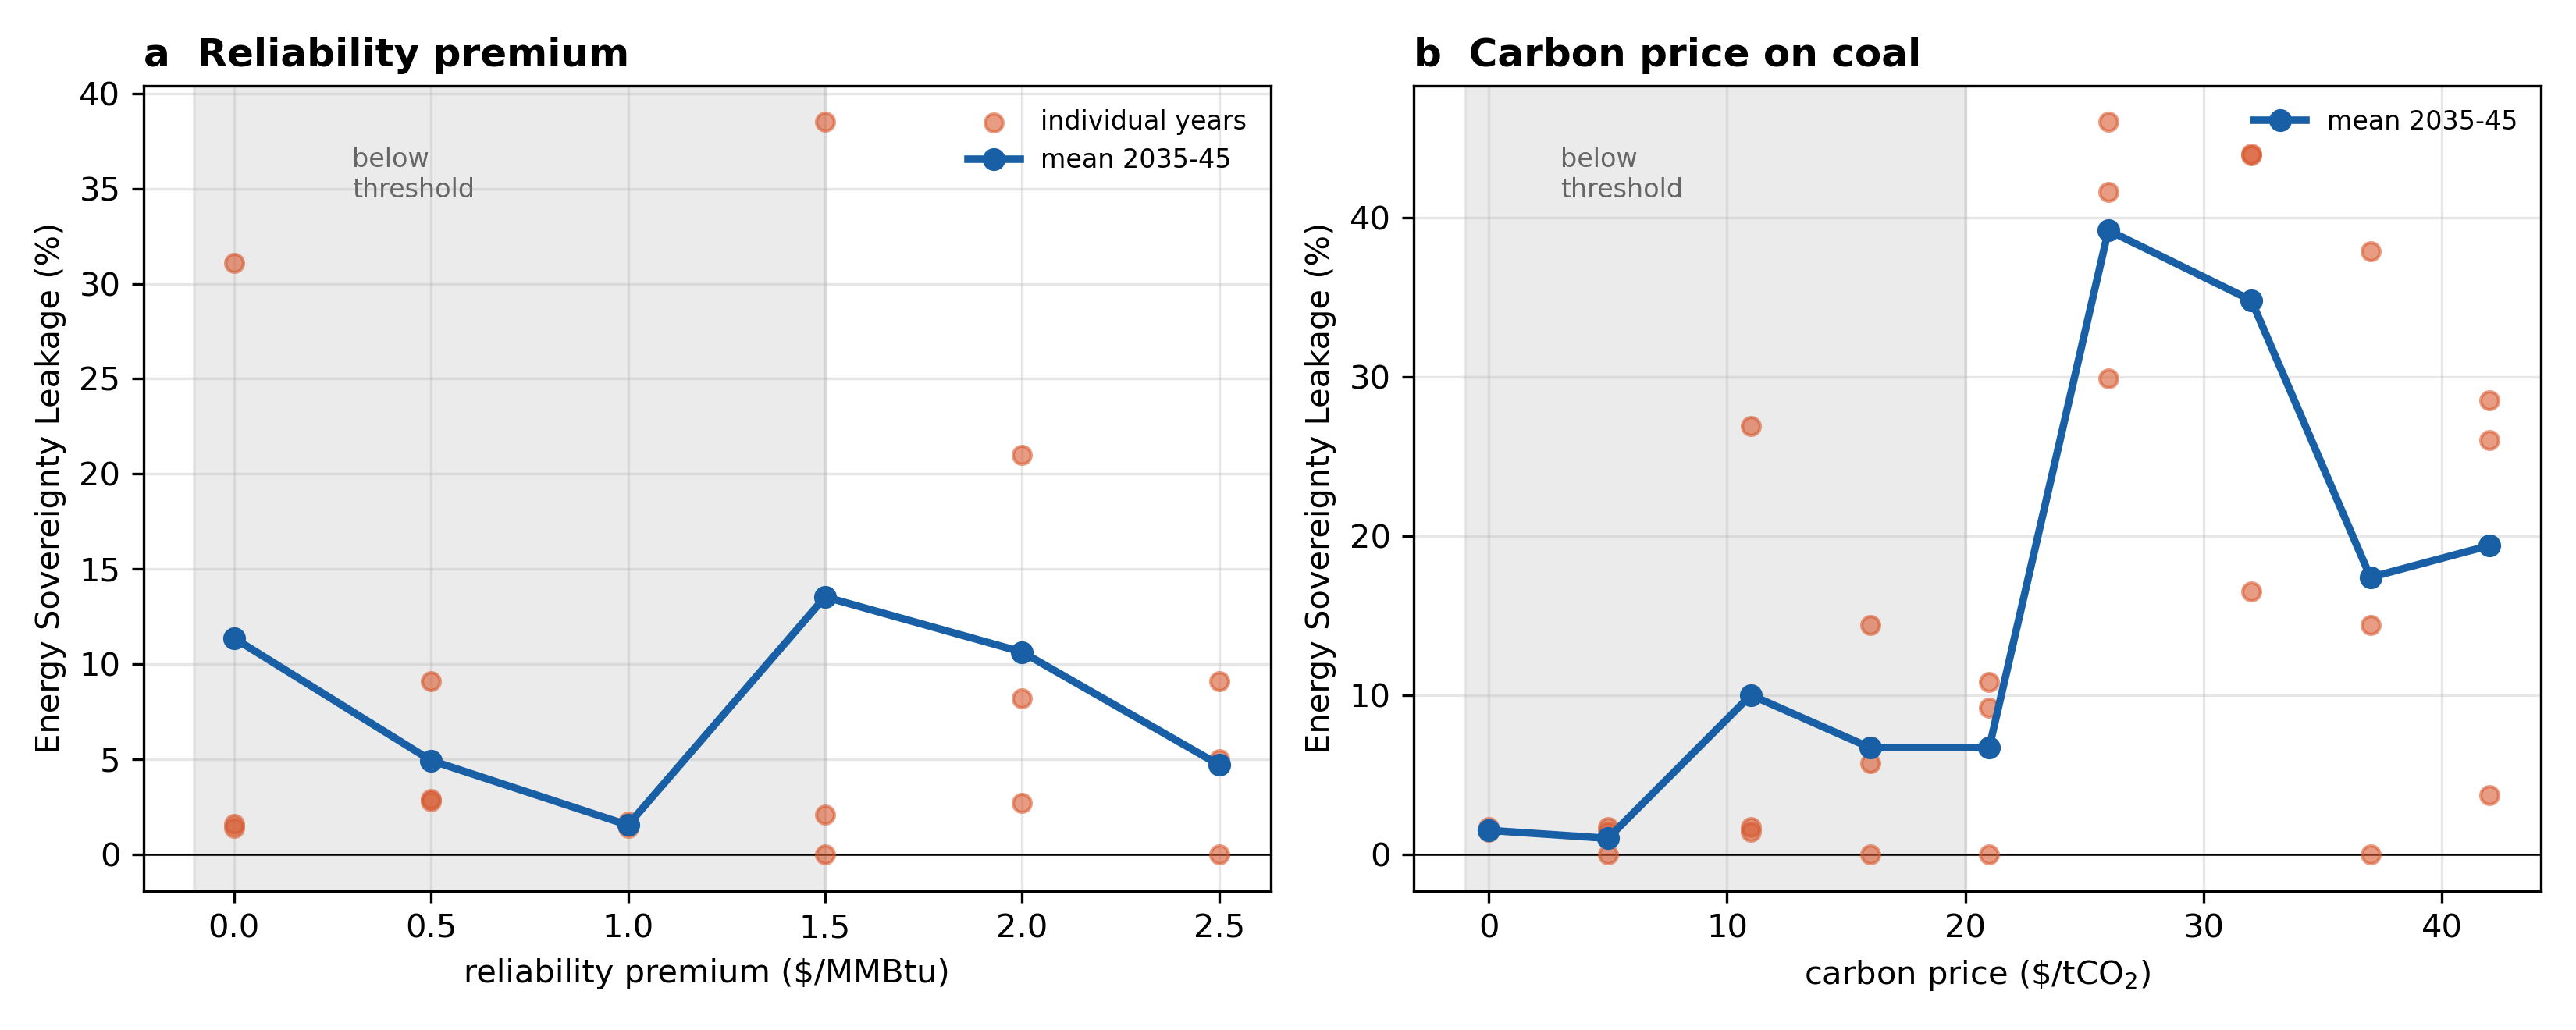
\includegraphics[width=0.7\linewidth]{outputs/figures/ESL_thresholds.png}
\caption{Leakage versus (a) the reliability premium $\rho$ and (b) the carbon
price $\tau$. In both, ESL is near zero below the crossing point and rises
steeply once delivered US LNG undercuts coal. The two axes are
mechanistically equivalent: each lowers the delivered-US-LNG-minus-coal
margin.}\label{fig:carbonsweep}
\end{figure}

% ---------------------------------------------------------------
\section{Scenario matrix and response surface}\label{si:scenario}

Beyond the threshold, the leaked magnitude is conditional. Supplementary
Figure~\ref{fig:heatmap} maps the headline ESL across US export capacity and
Mexican-shale cost; ESL is governed almost entirely by US export capacity and
is essentially flat in Mexican-shale cost, confirming that the sovereignty
premium falls on Mexico rather than altering the global leak.

\begin{figure}[H]\centering
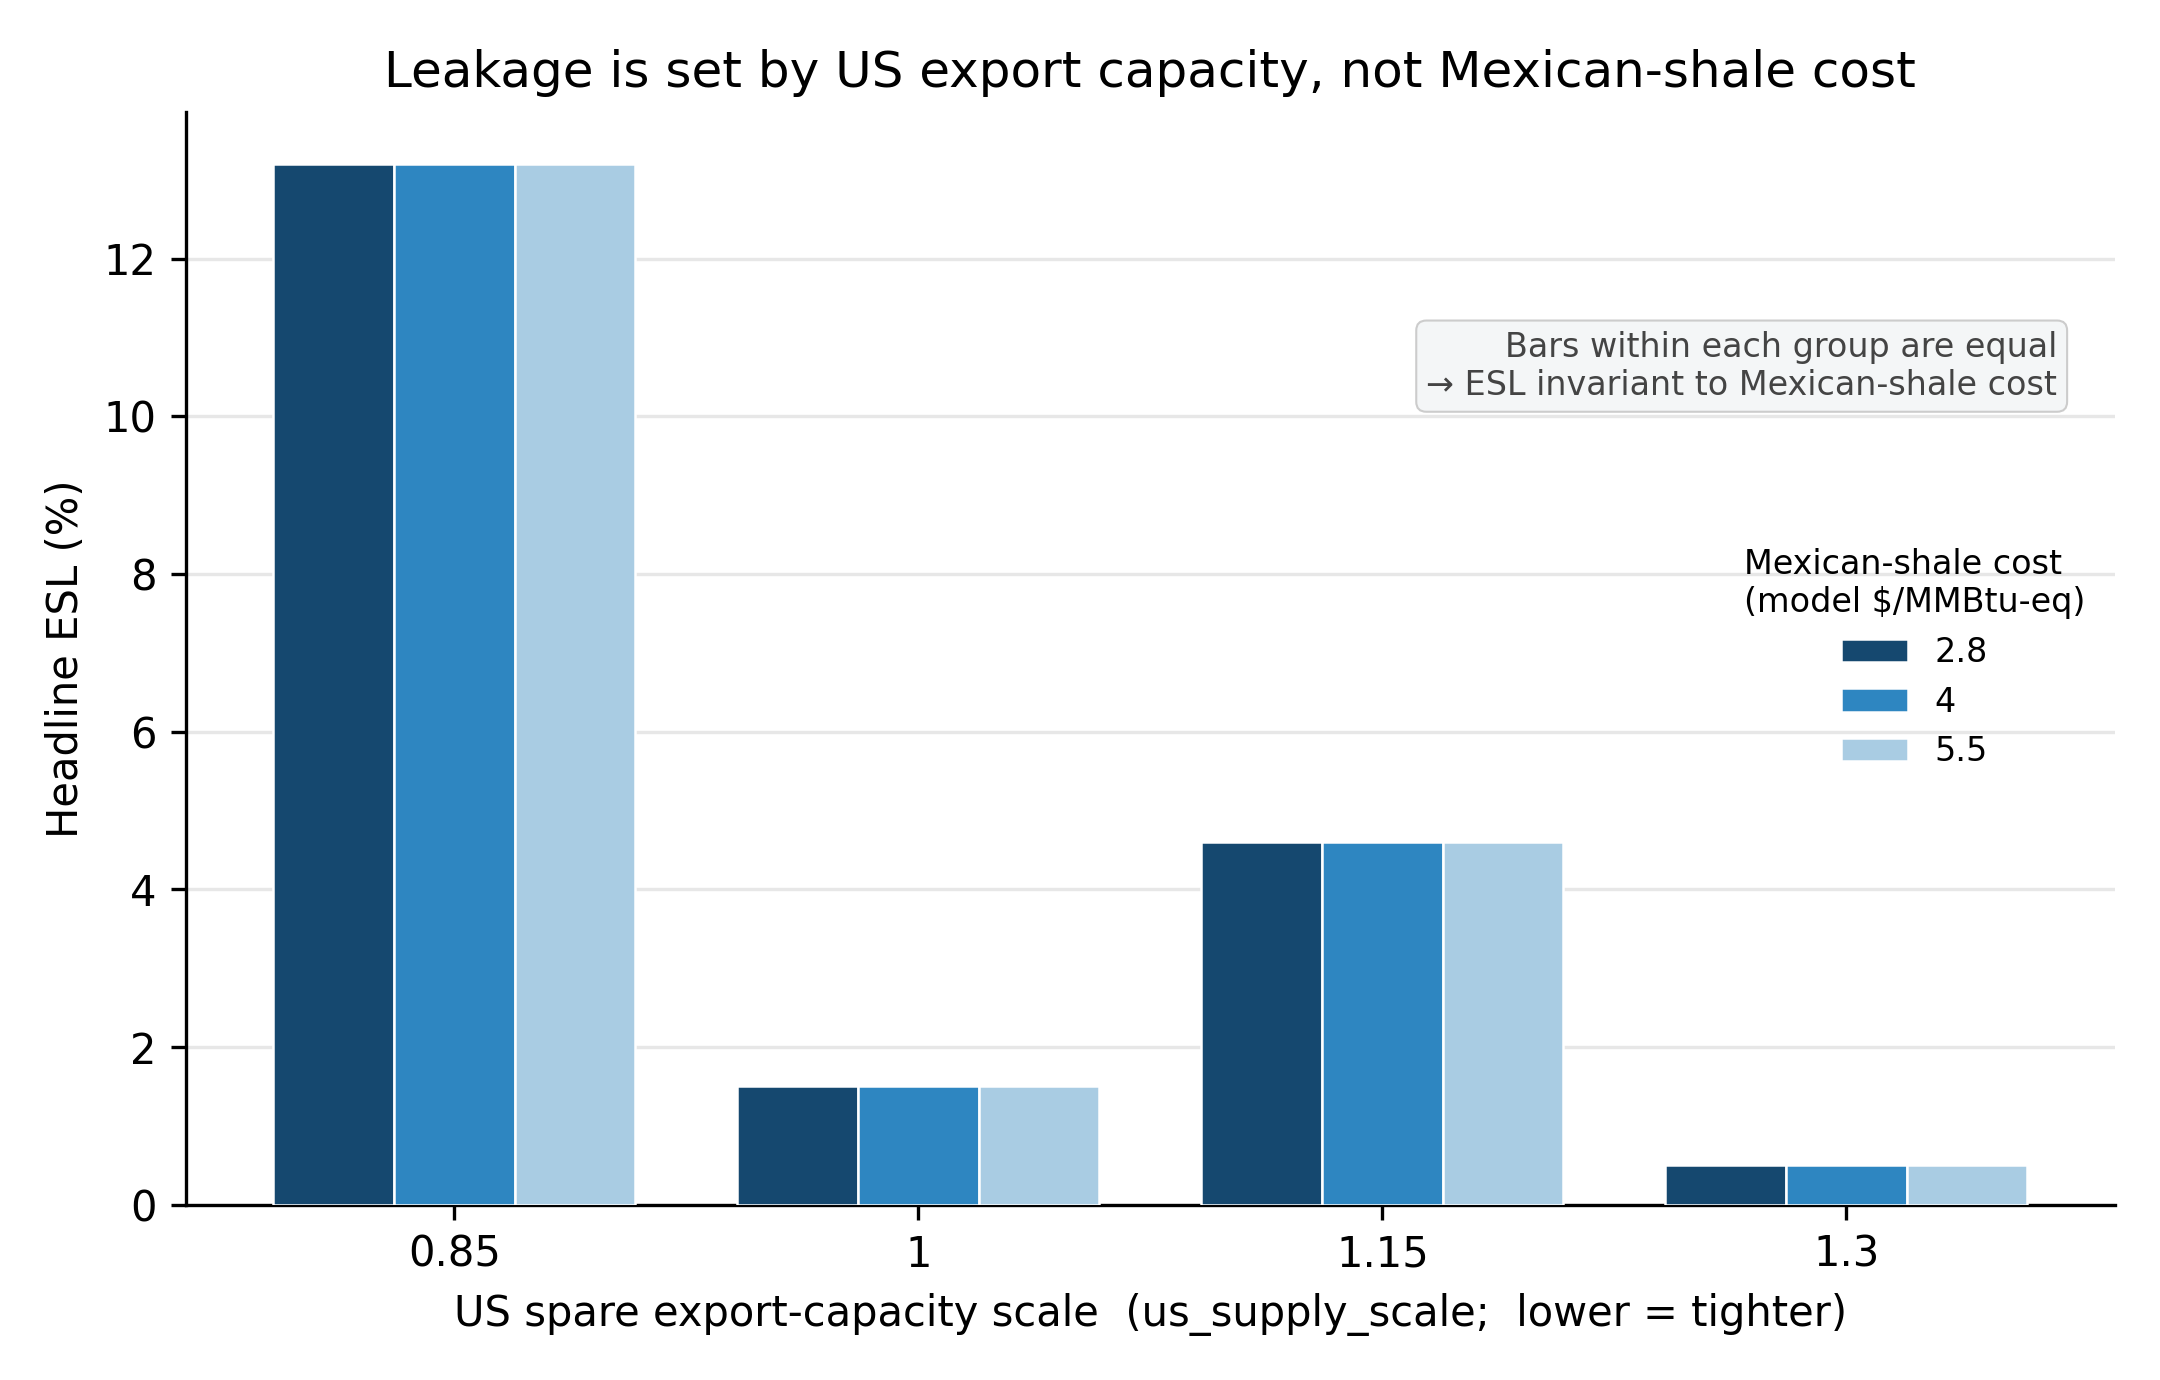
\includegraphics[width=0.7\linewidth]{outputs/figures/Scenario_heatmap.png}
\caption{Headline ESL across US spare export capacity
(\texttt{us\_supply\_scale}) and the cost of Mexican shale, shown as grouped
bars. Within each capacity group the three Mexican-shale-cost bars are
identical, so leakage is invariant to Mexican-shale cost; across groups leakage
rises as US spare capacity \emph{tightens} (lower \texttt{us\_supply\_scale}).
The non-monotonic step at the central scale reflects the discrete,
market-by-market tipping of the least-cost switch that makes the
above-threshold magnitude conditional.}\label{fig:heatmap}
\end{figure}

% ---------------------------------------------------------------
\section{Parameter uncertainty}\label{si:uncertainty}

A Monte Carlo over the governing cost, methane and capacity parameters
(triangular distributions, low/central/high in Table~\ref{tab:params};
\texttt{N\_MONTECARLO}~$=200$ for the final run) yields the distribution of
headline ESL, and a one-at-a-time tornado ranks the parameters by influence
(Supplementary Fig.~\ref{fig:uncertainty}). The tornado confirms that leakage is
governed by the delivered-LNG cost stack---liquefaction cost and coal parity---
and by US export capacity, and is weakly sensitive to the cost of Mexican shale;
the Monte Carlo distribution is concentrated near zero under present-day prices,
with its upper tail corresponding to the above-threshold regime.

\begin{figure}[H]\centering
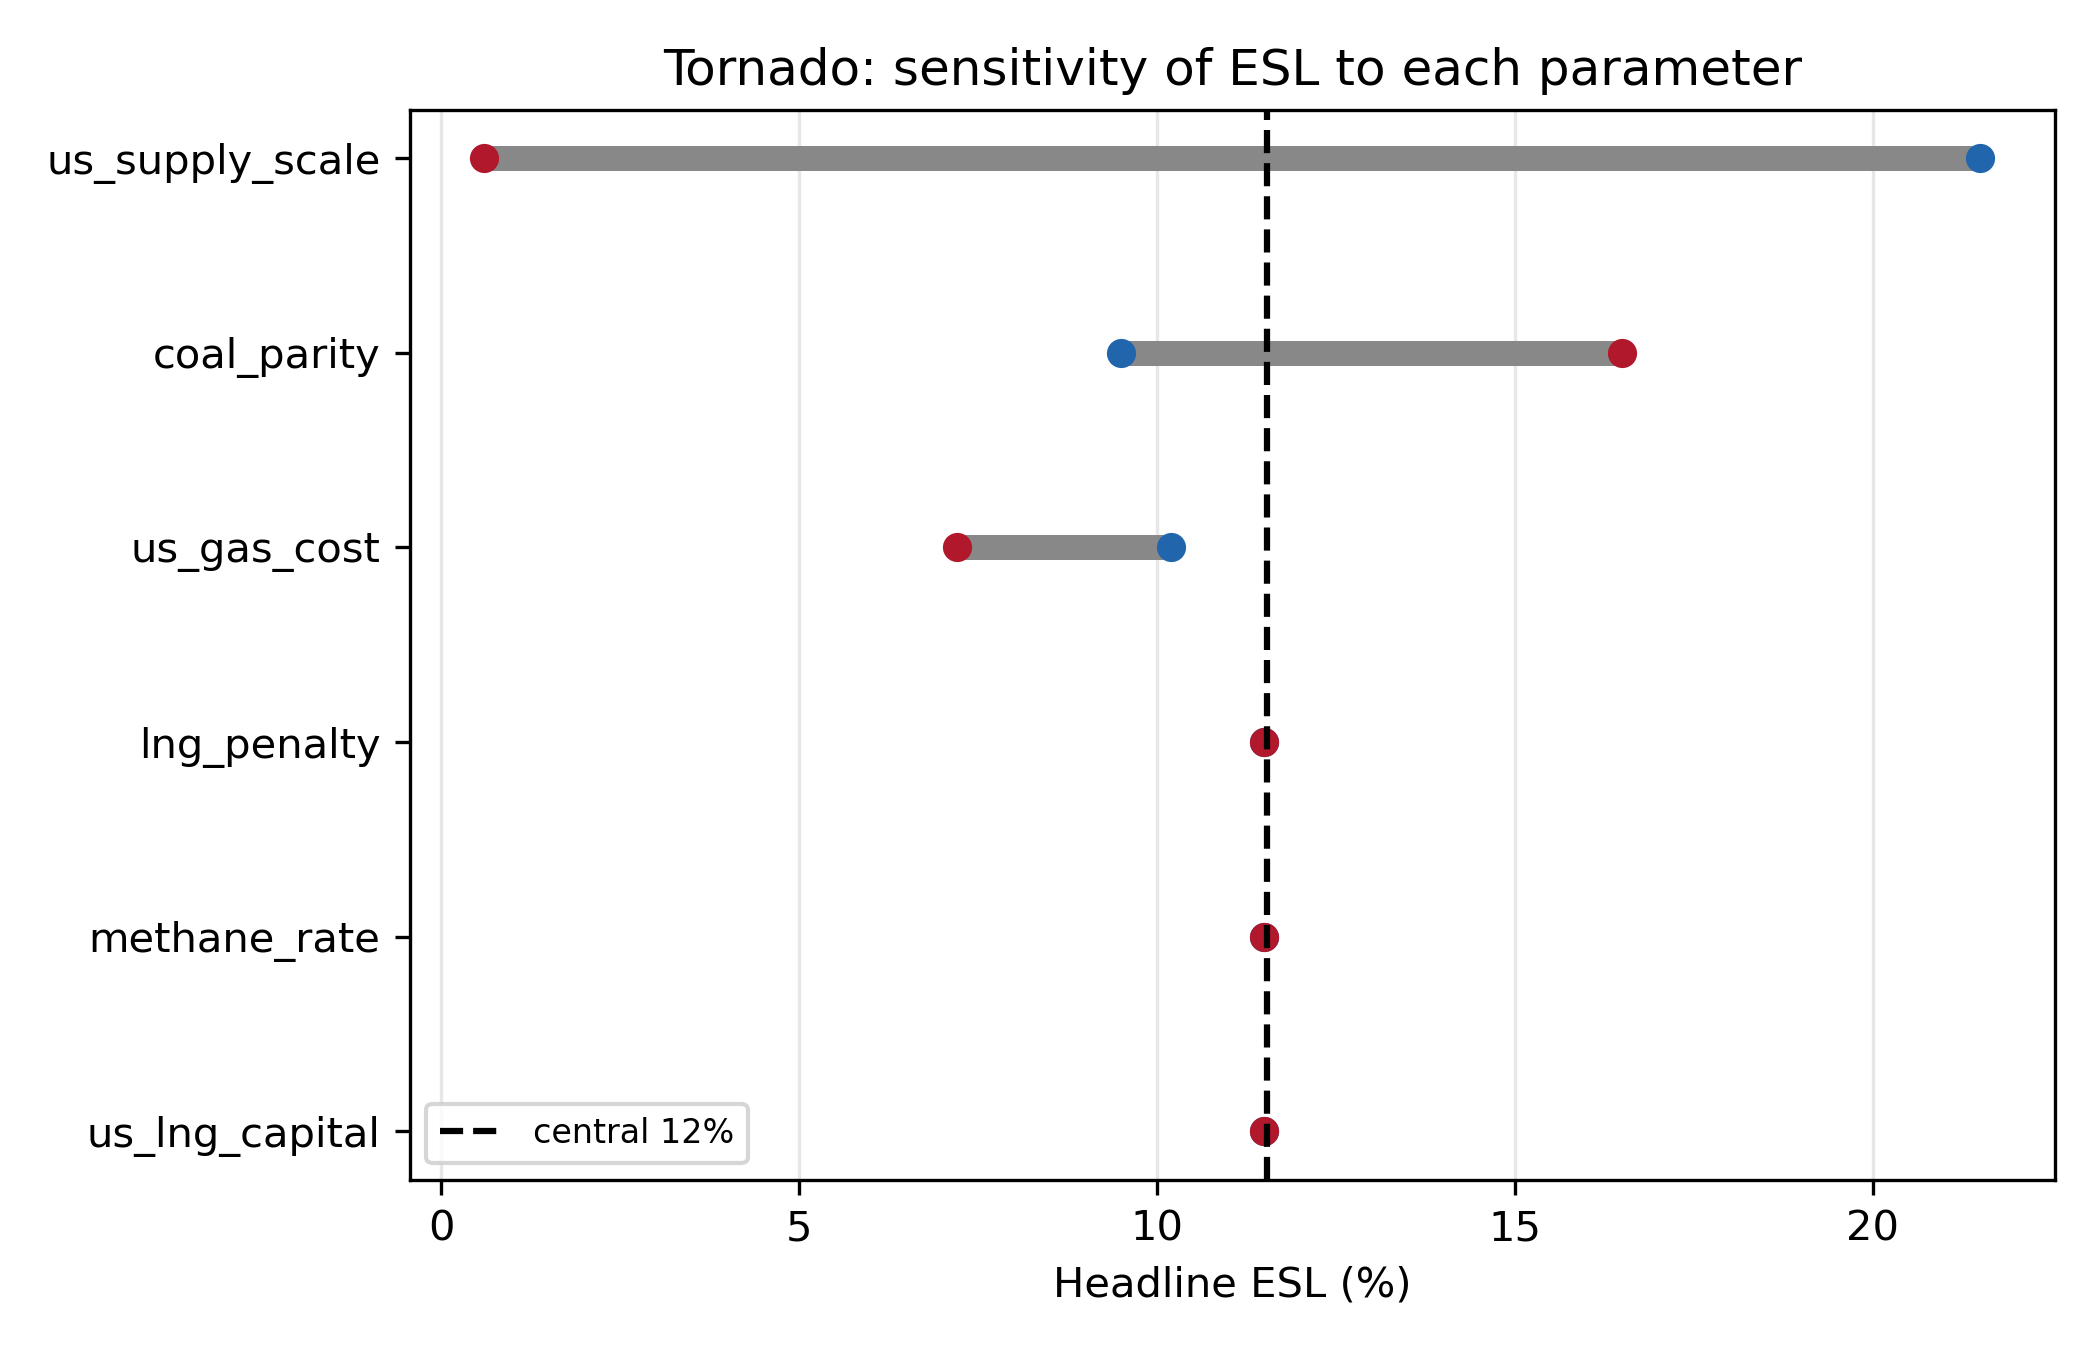
\includegraphics[width=0.49\linewidth]{outputs/figures/Uncertainty_tornado.png}
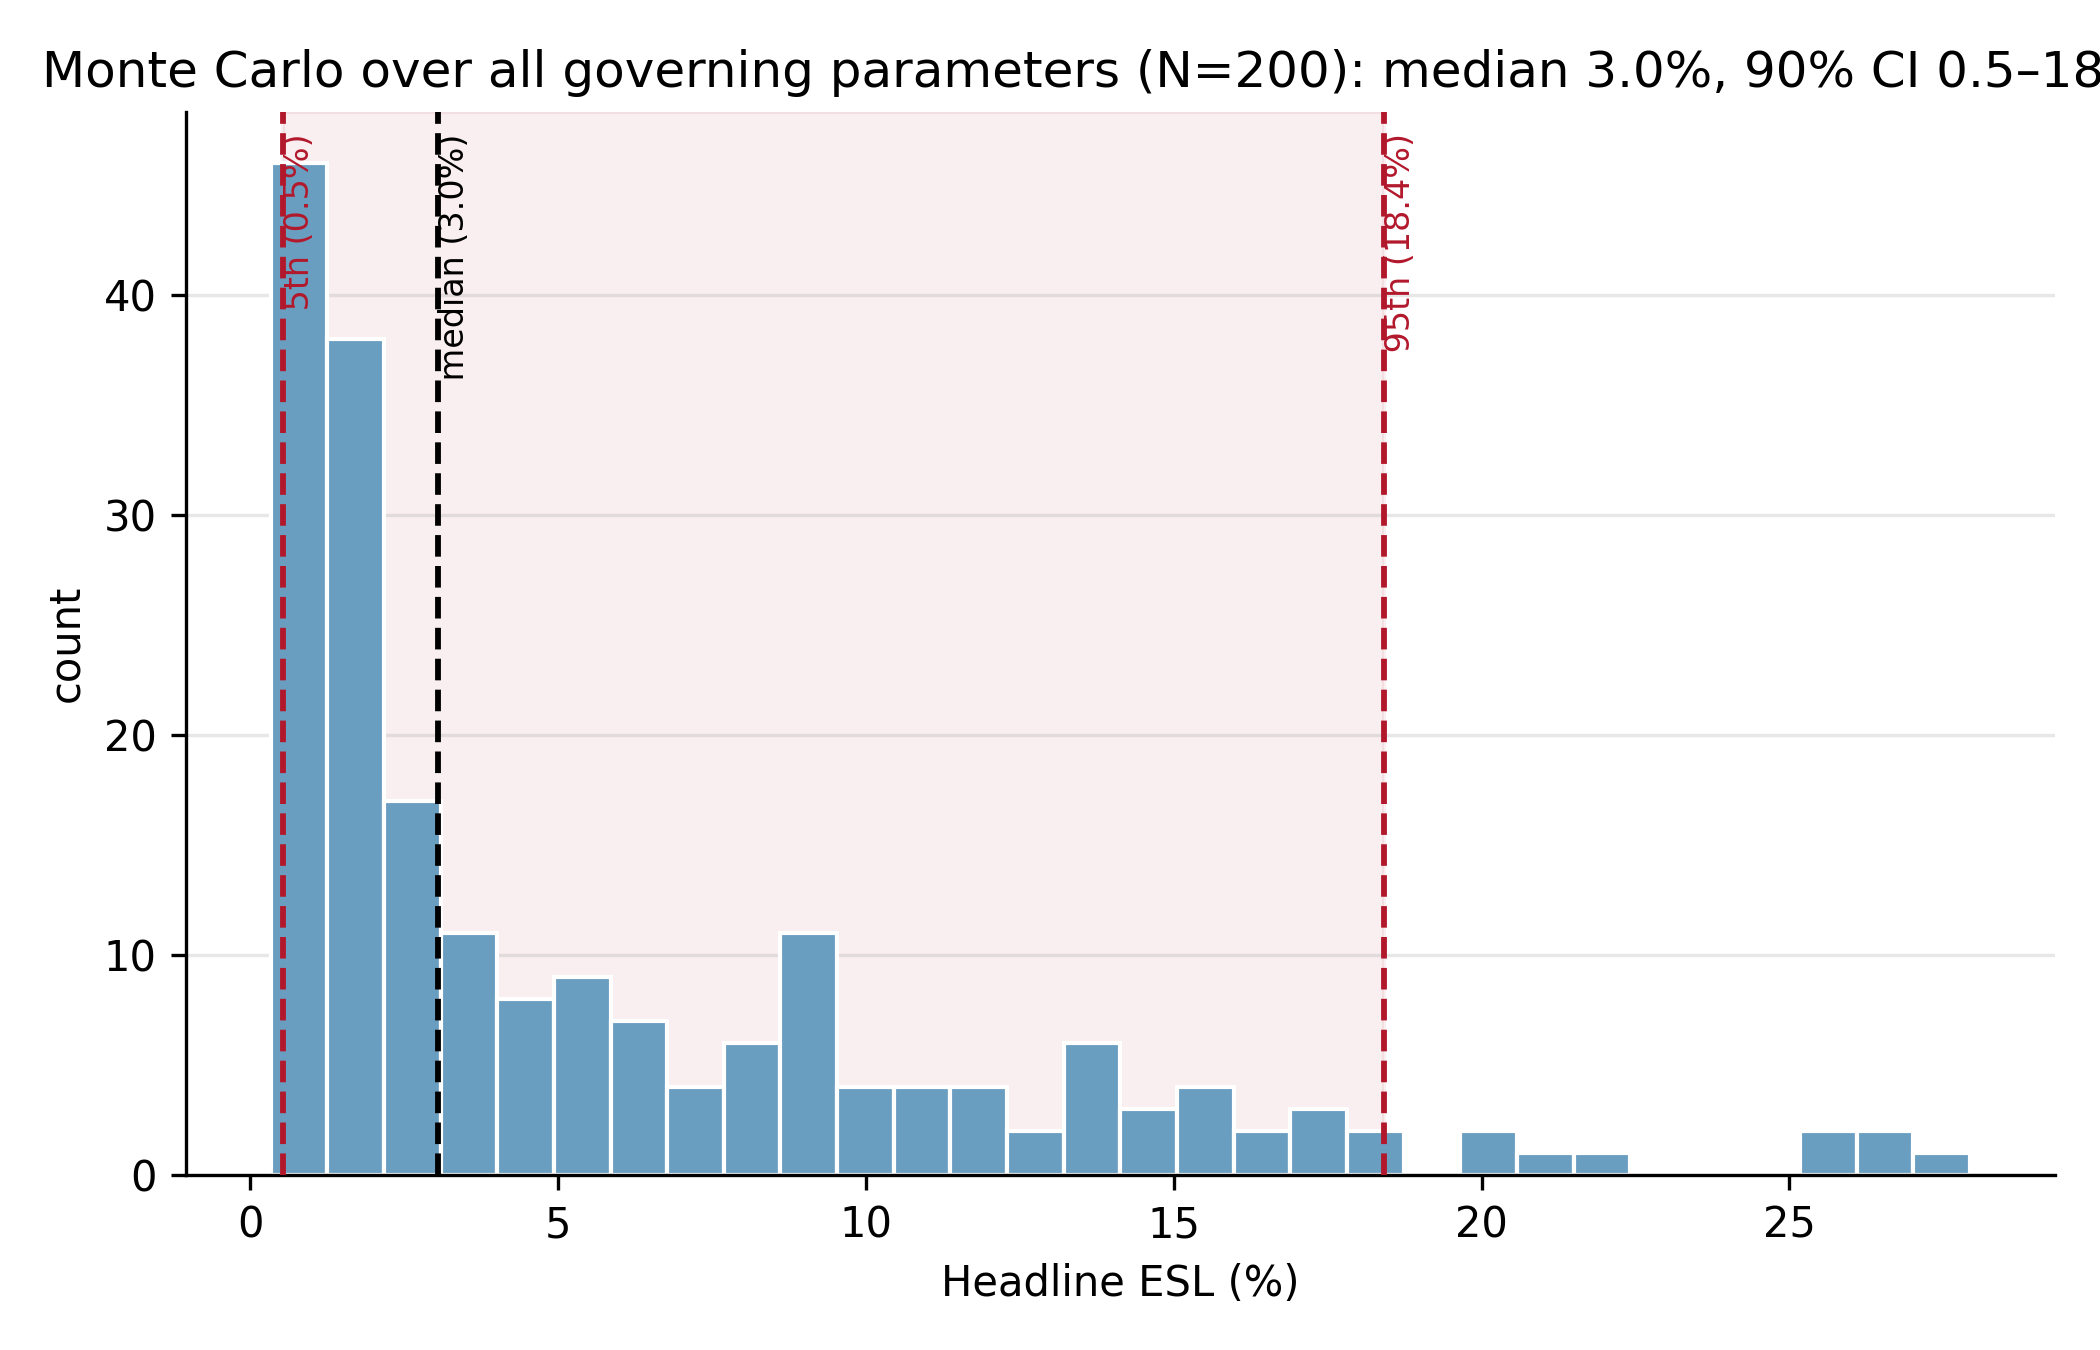
\includegraphics[width=0.49\linewidth]{outputs/figures/Uncertainty_montecarlo.png}
\caption{Left: tornado sensitivity of headline ESL to each parameter; leakage
is governed by the delivered-LNG cost stack (liquefaction cost, coal-parity)
and US export capacity. Right: Monte Carlo distribution of headline ESL
across all parameters.}\label{fig:uncertainty}
\end{figure}

% ---------------------------------------------------------------
\section{Global sensitivity, structural robustness and break-even levers}\label{si:robust}

Three further analyses, all from the same model, separate what governs the
leakage \emph{threshold} from what governs its \emph{magnitude}, and test the
parameters that set the coal-parity wall.

\paragraph{Global sensitivity.} A variance-based (standardised-regression)
sensitivity over all governing parameters ranks their influence on headline ESL
(Supplementary Fig.~\ref{fig:sensglobal}). US spare export capacity
(\texttt{us\_supply\_scale}, $|\beta|=0.46$) and the US gas cost ($0.22$)
dominate; the coal-parity level ($0.09$) and LNG-chain penalty ($0.06$) enter as
the delivered-cost stack predicts; the upstream methane rate ($0.03$) and the
US-LNG capital adder ($0.01$) are minor \emph{for the leaked volume}---methane
governs the climate \emph{sign}, not the quantity of gas that moves. Leakage is
thus controlled by the parameters that set where delivered US LNG sits relative
to the coal-parity wall, as the threshold mechanism predicts, and is nearly
insensitive to the Mexican-shale cost (Supplementary Fig.~\ref{fig:heatmap}).

\begin{figure}[H]\centering
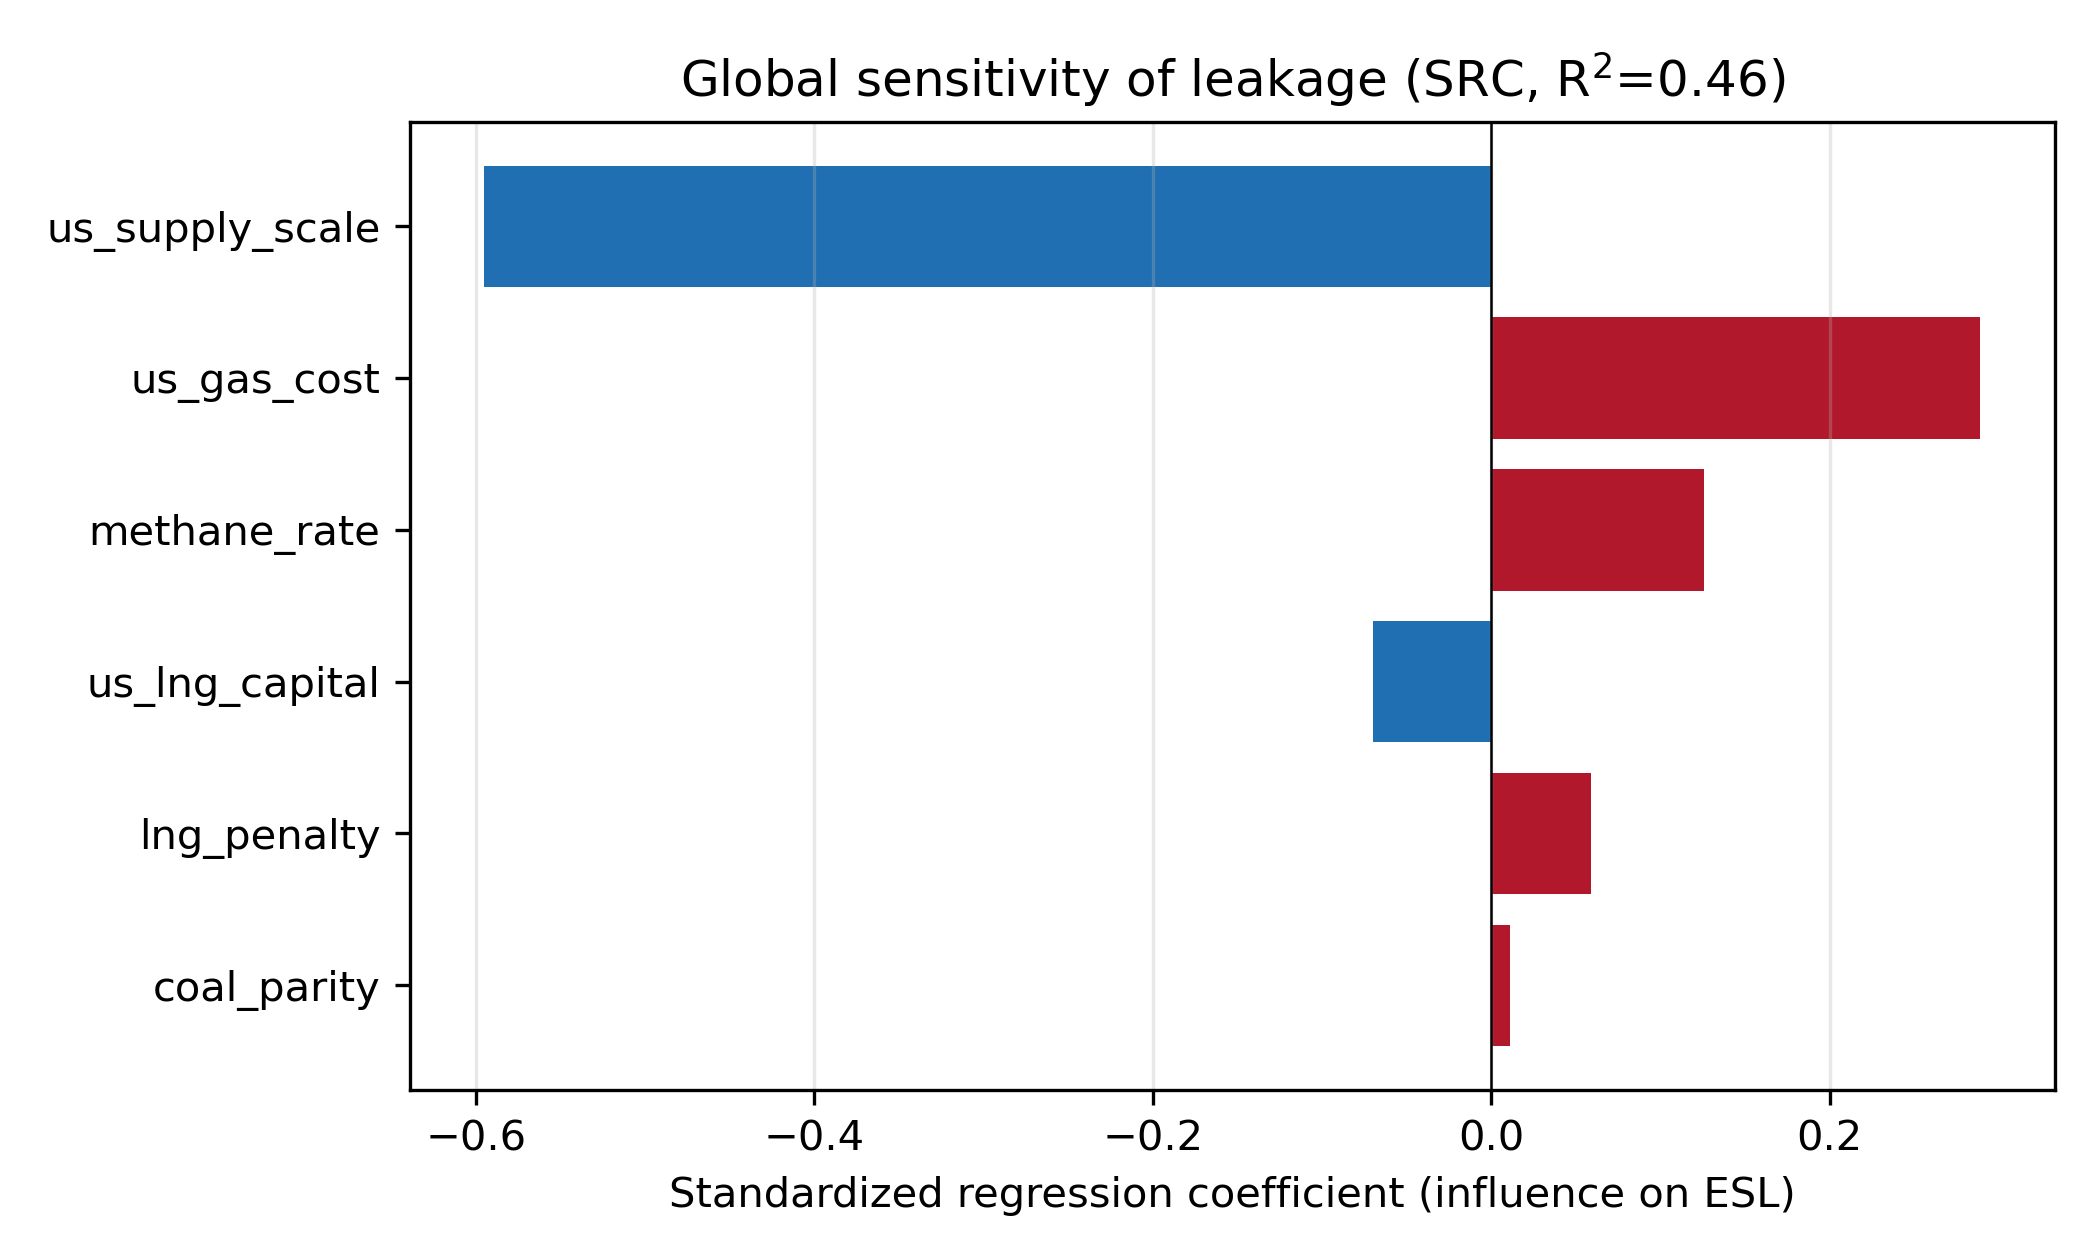
\includegraphics[width=0.68\linewidth]{outputs/figures/Sensitivity_global.png}
\caption{Global sensitivity of headline ESL: standardised regression
coefficients (absolute value) for each governing parameter. US export capacity
and US gas cost dominate; coal-parity and LNG-chain cost are secondary; the
methane rate and LNG capital adder are minor for the leaked volume.}\label{fig:sensglobal}
\end{figure}

\paragraph{Structural robustness.} Disabling individual model components
isolates their effect (Supplementary Fig.~\ref{fig:senstoggle}). The central
near-zero result depends on the demand representation: with price-elastic demand
disabled, headline ESL rises from $\sim$1\% to $\sim$14\%, because part of the
freed volume is then forced through trade rather than absorbed by lower Mexican
consumption---so the elastic-demand case is the conservative one. Removing the
depletion curve (flat US supply) raises ESL to $\sim$4\%. A pure linear program
(no quadratic convexity) collapses baseline leakage to zero, the degeneracy that
motivated the convex reformulation. These bounds identify demand elasticity and
the supply-curve shape, not the solver, as the structural choices that matter.

\begin{figure}[H]\centering
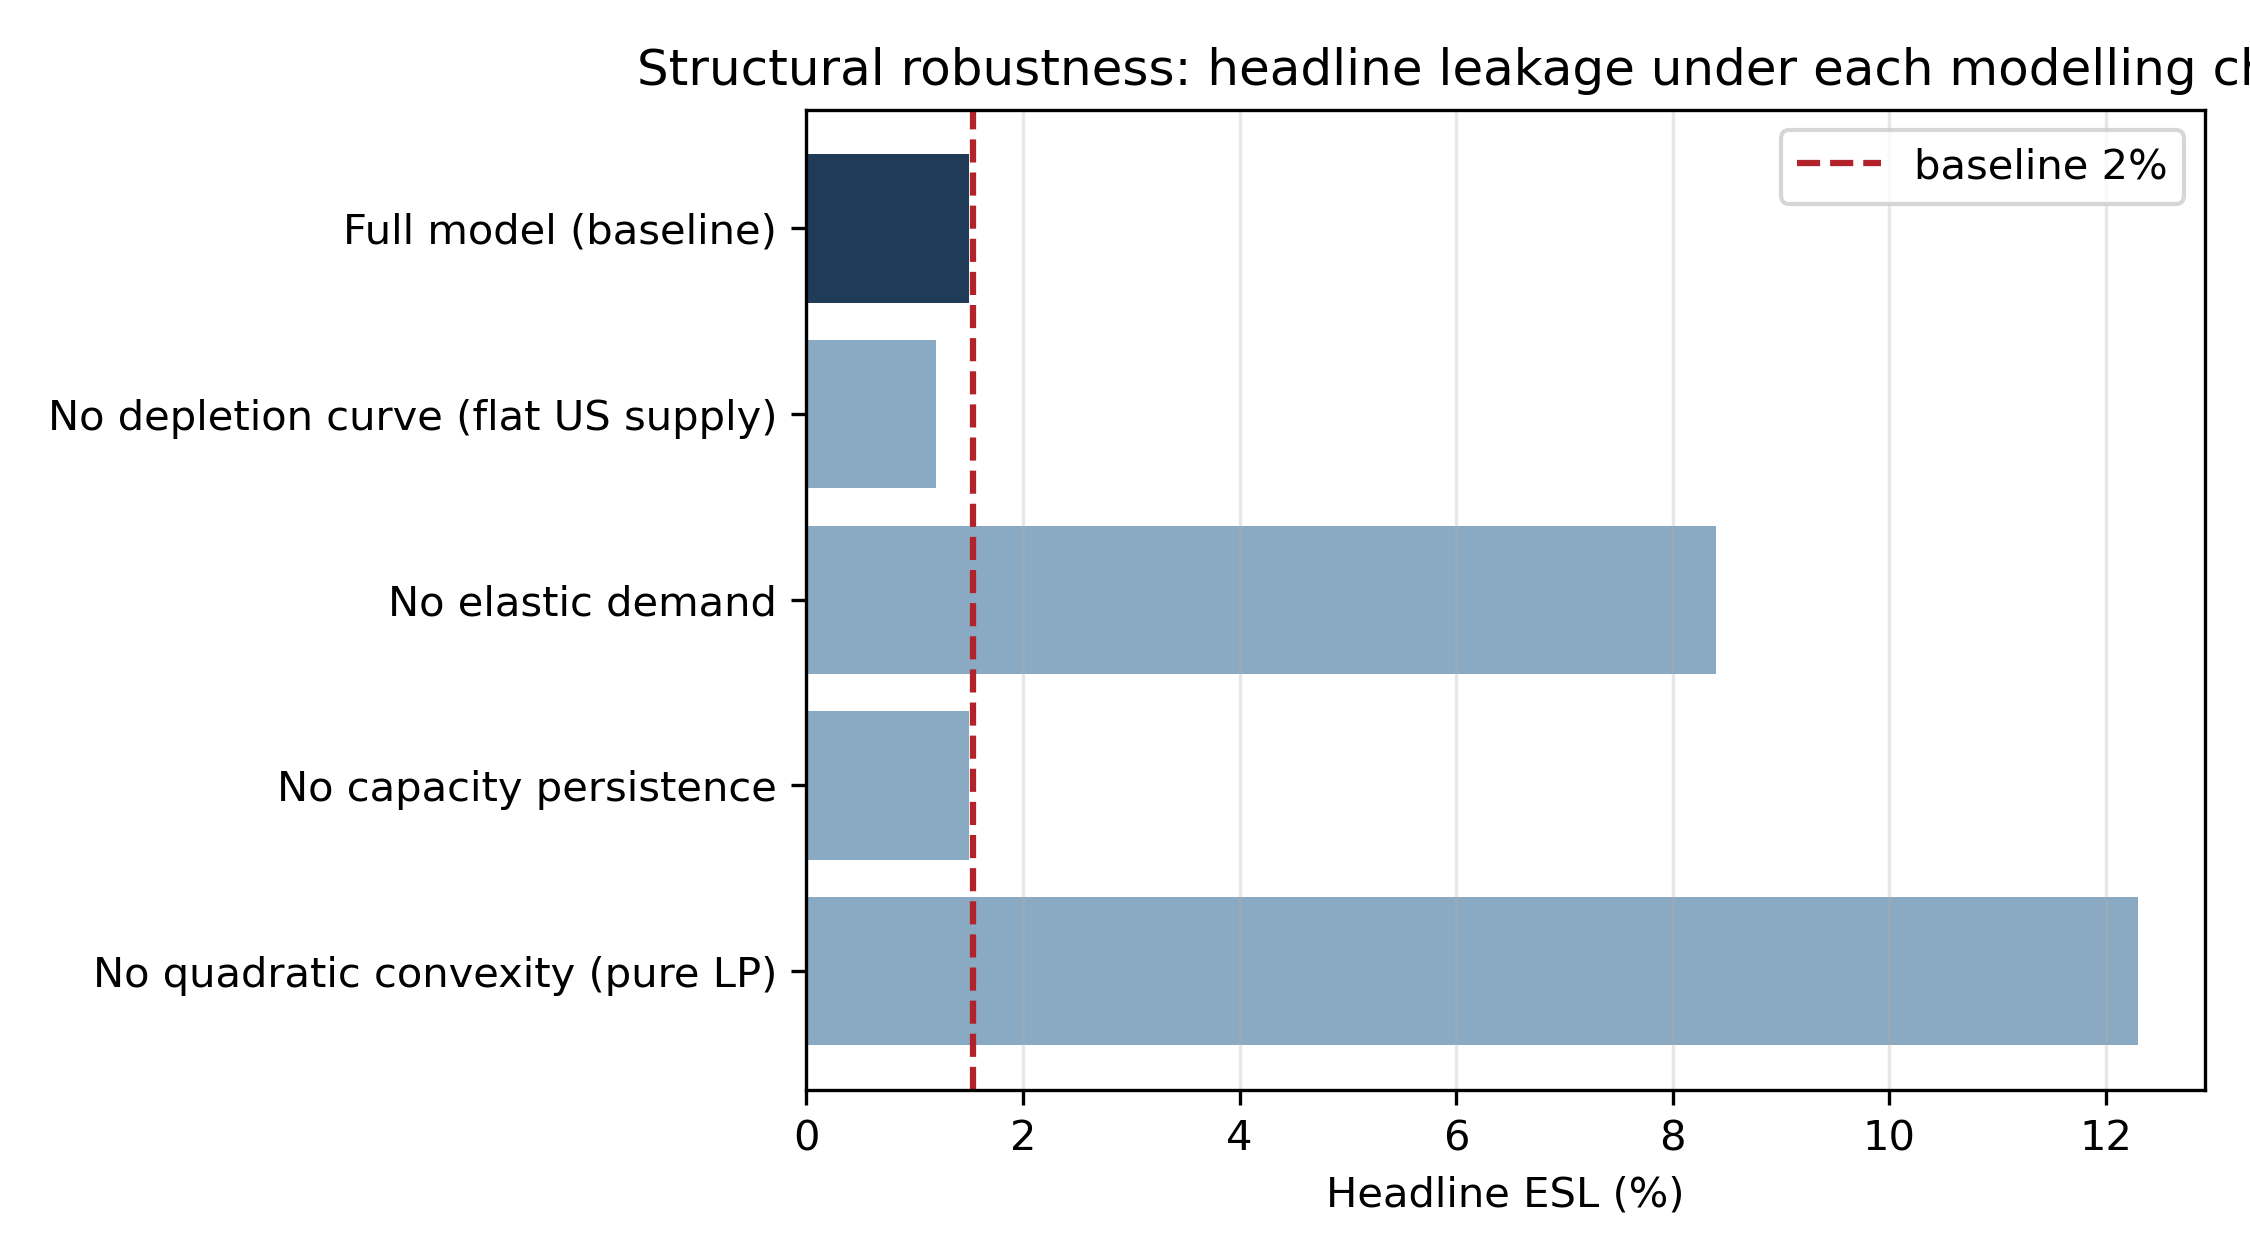
\includegraphics[width=0.68\linewidth]{outputs/figures/Sensitivity_toggle.png}
\caption{Structural robustness: headline ESL under successive removal of model
components. Demand elasticity and the US depletion curve are the influential
structural choices; the pure-LP case exposes the degeneracy the quadratic
convexity term removes.}\label{fig:senstoggle}
\end{figure}

\paragraph{Break-even levers.} We report the value of each policy lever at which
above-threshold leakage reaches a reference 25\% share
(Table~\ref{tab:breakeven}). A tightening of US spare export capacity to
$0.83\times$ the central level carries the system to that share; within the swept
ranges neither the reliability premium nor a carbon price alone reaches a 25\%
mean (each drives leakage into the low tens of percent), consistent with the
global-sensitivity ordering that places US supply first. The
crossing \emph{locations} are well determined even where the leaked magnitude
beyond them is not, which is why we treat the threshold, not a percentage, as
the result.

\begin{table}[H]\centering
\caption{Break-even value of each lever at which above-threshold leakage reaches
a 25\% reference share (\texttt{src/sensitivity.py}).}\label{tab:breakeven}
\begin{tabular}{@{}lll@{}}
\toprule
Lever & Unit & Value for 25\% ESL \\
\midrule
US spare-capacity scale    & $\times$ central          & 0.83 \\
Reliability premium $\rho$ & \$/MMBtu                 & no crossing within range \\
Carbon price $\tau$        & \$/tCO\textsubscript{2}   & no crossing alone \\
\bottomrule
\end{tabular}
\end{table}

\paragraph{The threshold is not an artefact of least-cost tipping.} A natural
concern is that the leakage threshold is manufactured by the discrete,
market-by-market switching of a least-cost merit order, and would disappear
under smooth inter-supplier substitution. We test this by isolating the
coal-to-gas switching channel and re-expressing it two ways over the same
delivered-cost margin $m$ (delivered US LNG minus the local coal-parity price;
\texttt{src/logit\_switching.py}): the least-cost rule of the main model, in
which each heterogeneous coal sub-fleet (\texttt{COAL\_PARITY\_SPREAD}) switches
when delivered gas falls below its own parity, and a \emph{logit} market share,
in which the same sub-fleet switches with continuous probability
$\sigma((\delta_k-m)/\tau)$. Under both rules leakage turns on as $m$ crosses
zero---the delivered-gas-equals-coal point---with half-plateau crossings at
$m=+0.32$ and $m=0.00$~\$/MMBtu respectively (Supplementary
Fig.~\ref{fig:logit}). The logit representation removes the discrete steps, and
hence the non-convergent above-threshold magnitude of the main results, but does
not move the threshold: the crossing is a property of the delivered-cost
comparison, not of the solver. Fully endogenising this switching in the
19-region model does not resolve the above-threshold \emph{magnitude} to a
stable value---consistent with the non-convergence we already report for the
least-cost case---which is why we treat the threshold crossing, not a leaked
percentage, as the robust result.

\begin{figure}[H]\centering
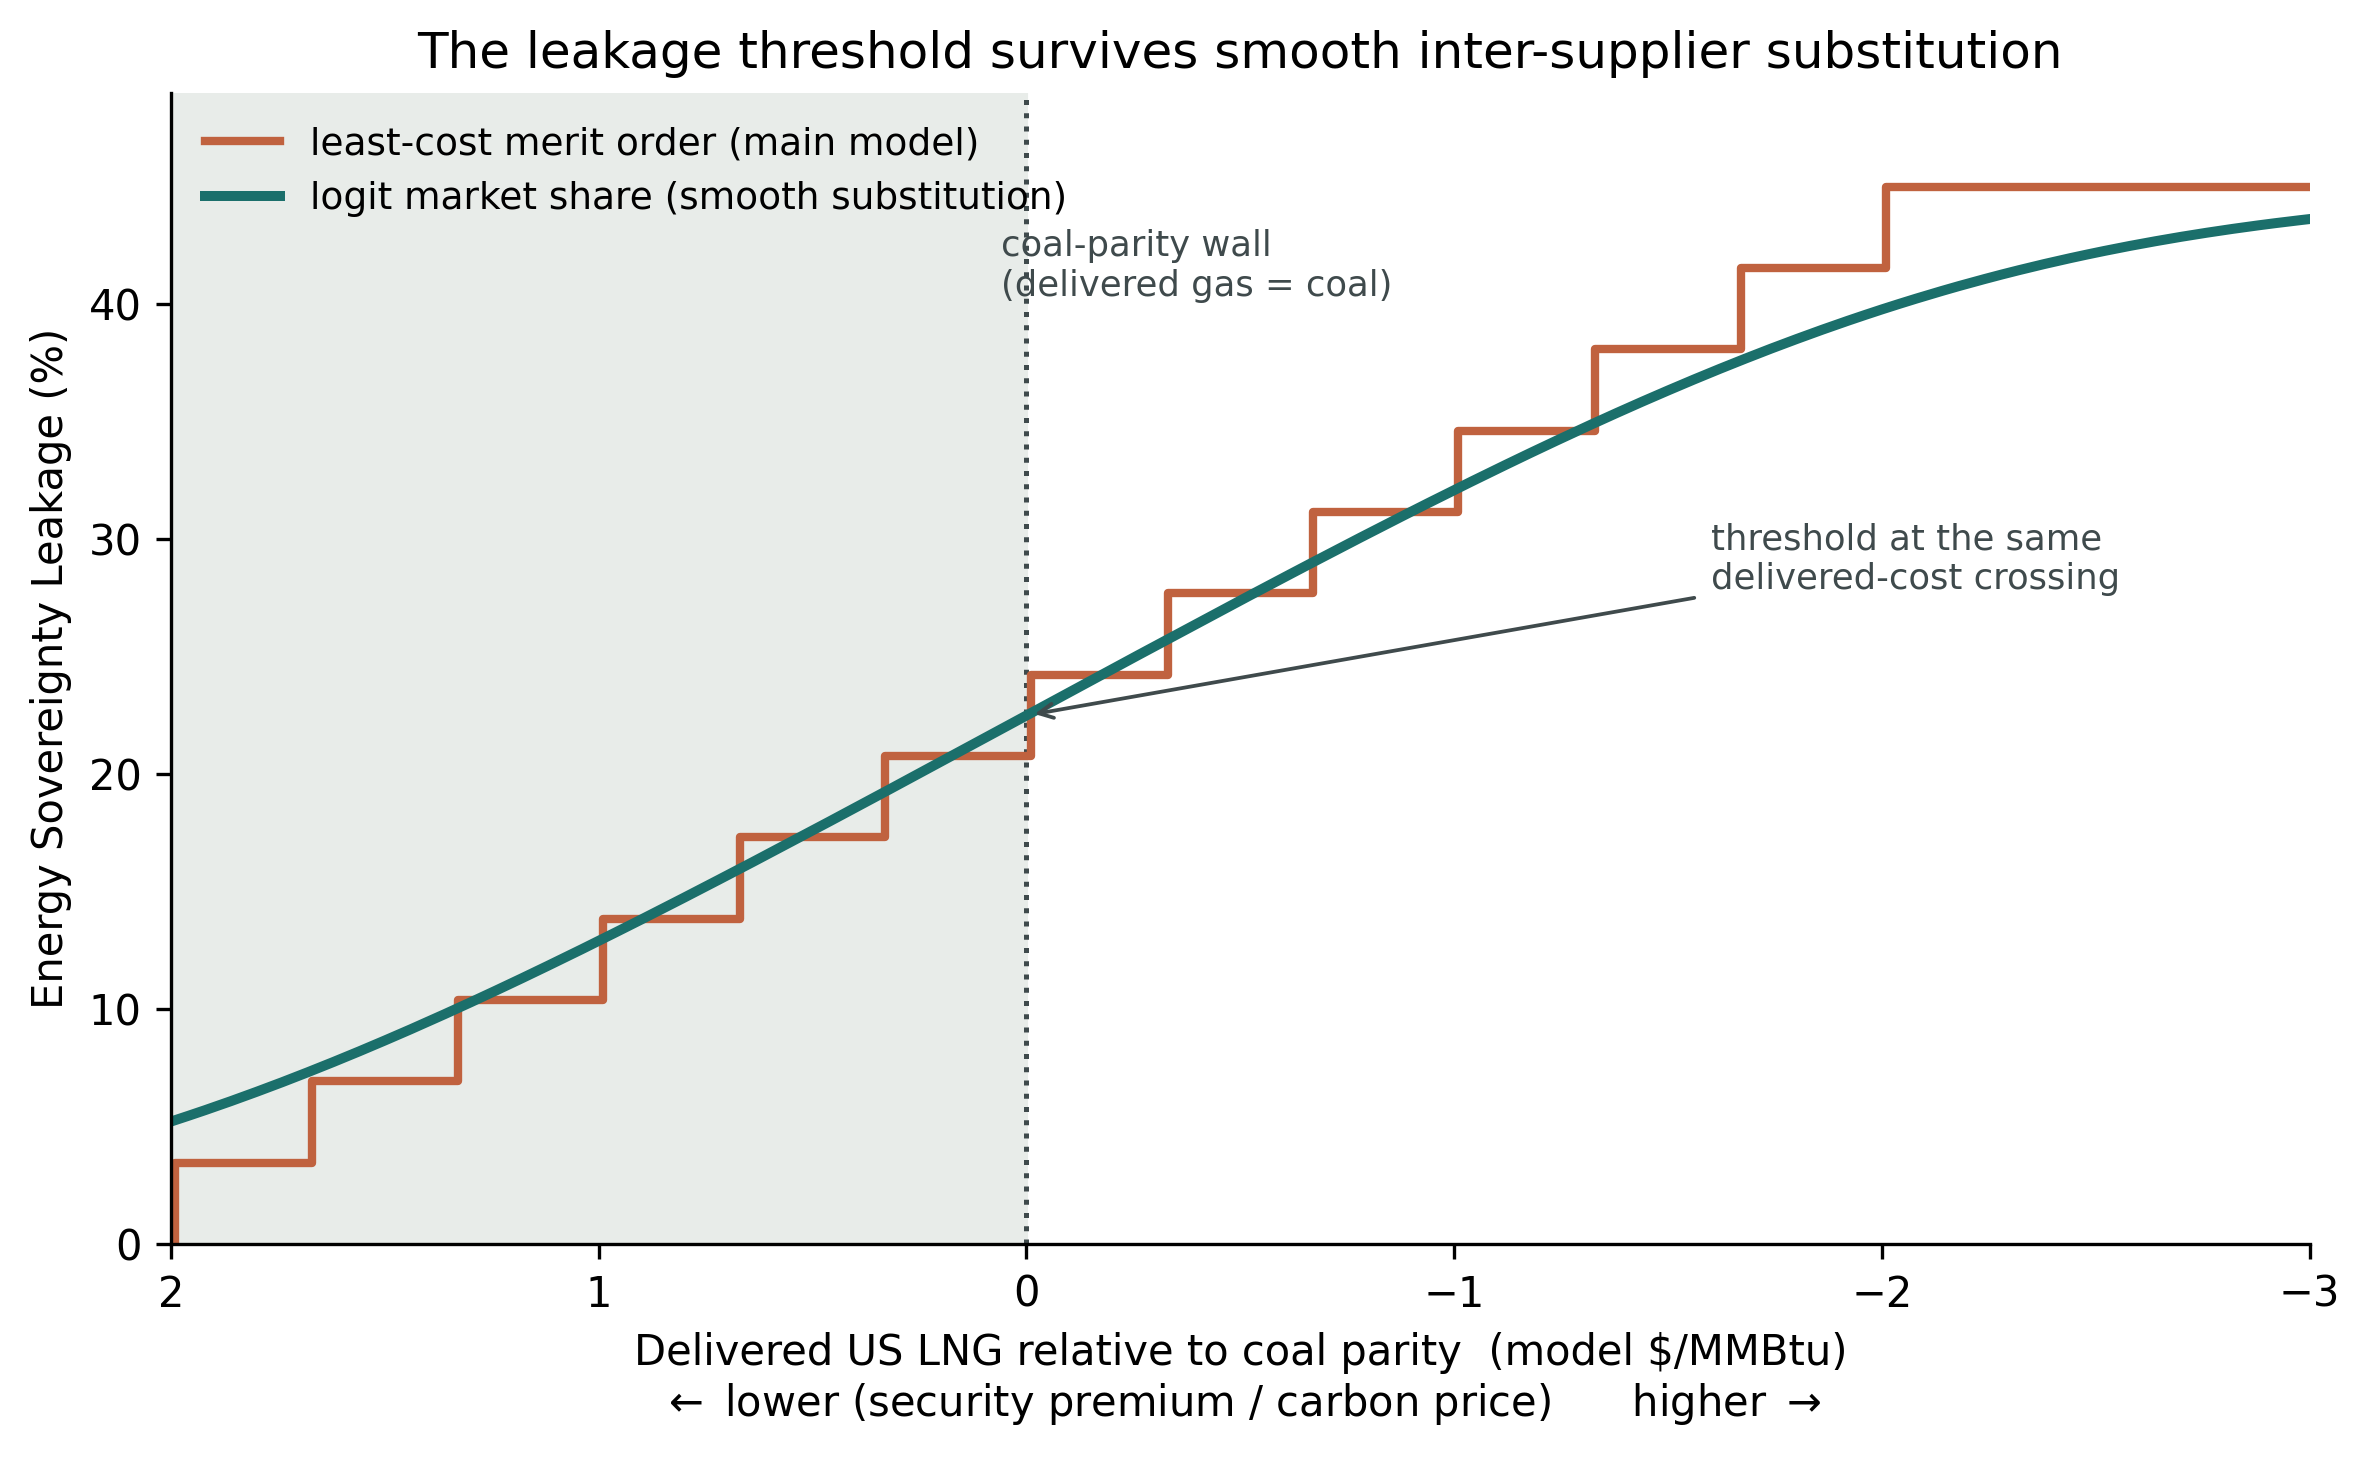
\includegraphics[width=0.78\linewidth]{outputs/figures/Threshold_logit_vs_leastcost.png}
\caption{Threshold robustness to the switching rule. Energy Sovereignty Leakage
from the coal-to-gas channel as a function of the delivered-cost margin (US LNG
relative to coal parity), under the main model's least-cost merit order (step)
and a smooth logit market share. Both switch on at the coal-parity wall
($m=0$); the logit rule smooths the magnitude without moving the threshold. The
plateau is scaled to the top of the main-model conditional range and is not the
object of the comparison---the coincident crossing is.}\label{fig:logit}
\end{figure}

% ---------------------------------------------------------------
\section{Regional supply, demand and trade}\label{si:regions_detail}

This section collects the region-resolved figures that complement those in the
main text. Gas demand diverges across regions
(Supplementary Fig.~\ref{fig:demandpanels}): Asian demand grows strongly while
European demand declines, which makes Asia the destination for freed gas once
the leakage threshold is crossed. US LNG destinations
(Supplementary Fig.~\ref{fig:lngdest}) show that US LNG serves Europe, Latin
America and a contracted volume to NE Asia (Japan and Korea), but does not
competitively reach the Chinese coal-switching market under present-day prices;
the net-trade positions
(Supplementary Fig.~\ref{fig:nettrade})
confirm that the sovereignty transition repositions who produces and who buys
rather than reducing global gas use; and resource depletion
(Supplementary Fig.~\ref{fig:reserves}) shows that sustained re-export
concentrates drawdown on the US unconventional base and a few established
exporters.

\begin{figure}[H]\centering
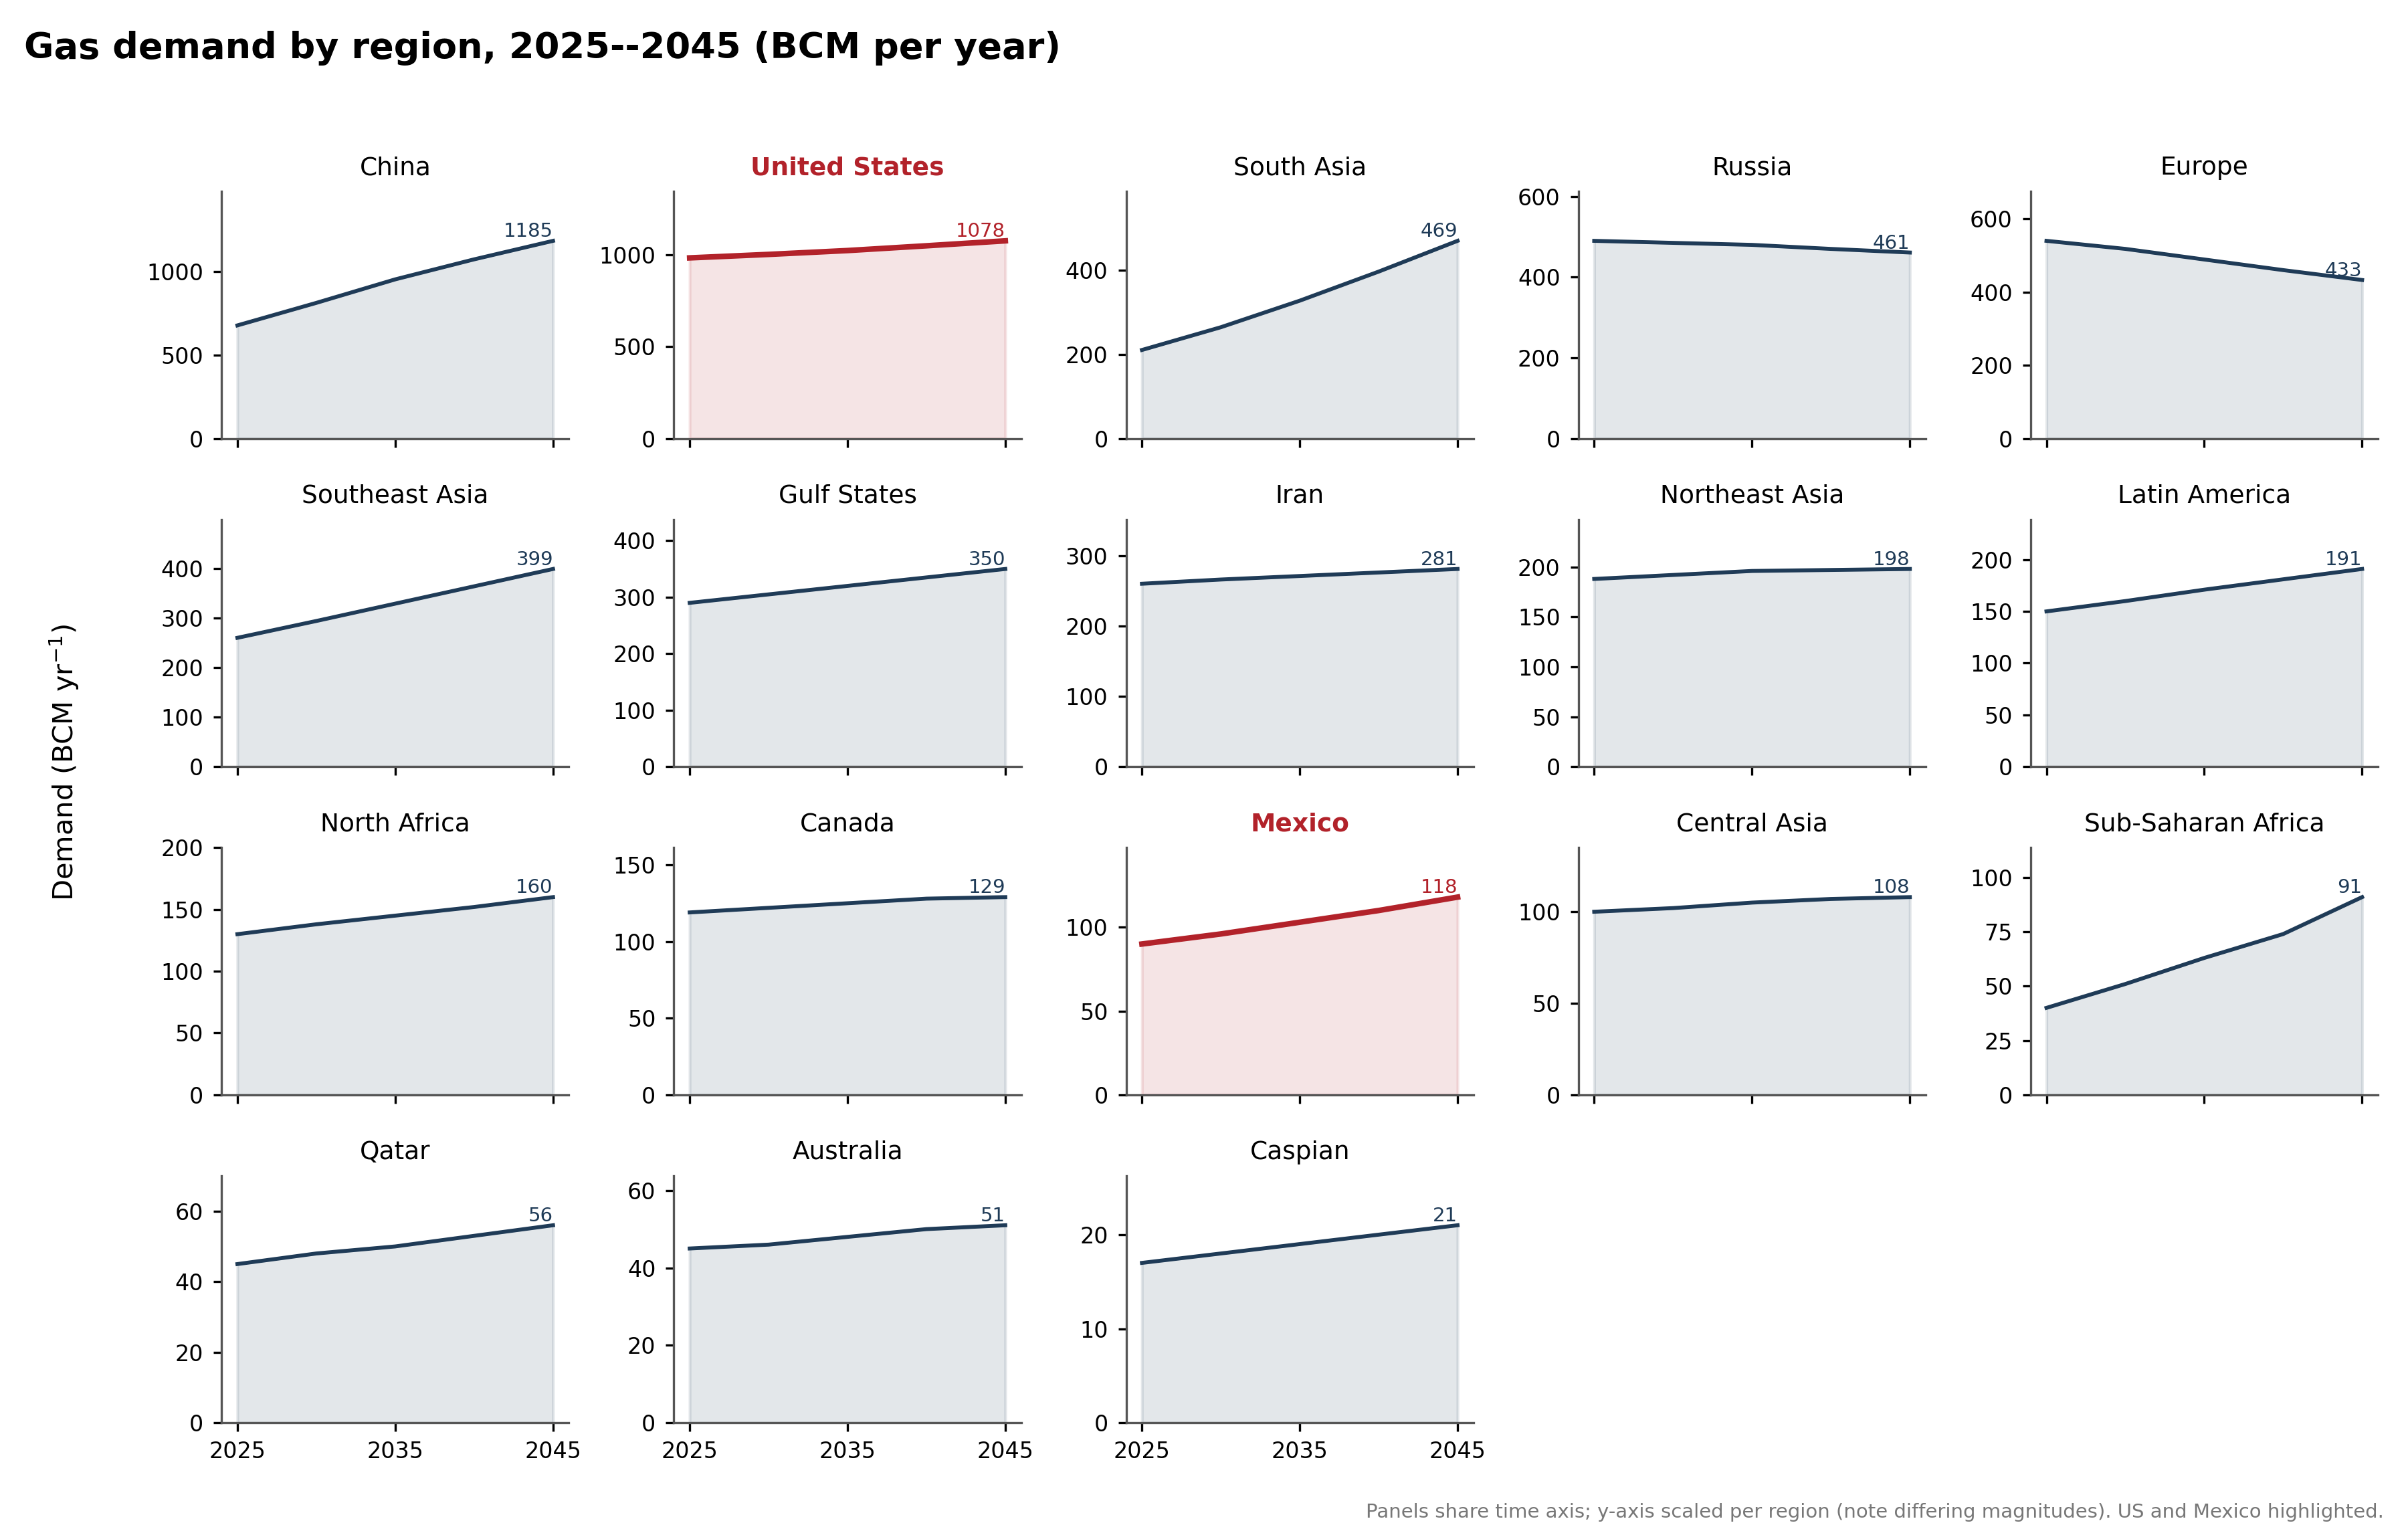
\includegraphics[width=\linewidth]{outputs/figures/Region_demand_panels.png}
\caption{Gas demand by region, 2025--2045 (BCM per year). Panels share the time
axis; the vertical axis is scaled per region, so compare trajectories rather
than absolute heights. Asian demand grows strongly while European demand
declines. United States and Mexico highlighted.}\label{fig:demandpanels}
\end{figure}

\begin{figure}[H]\centering
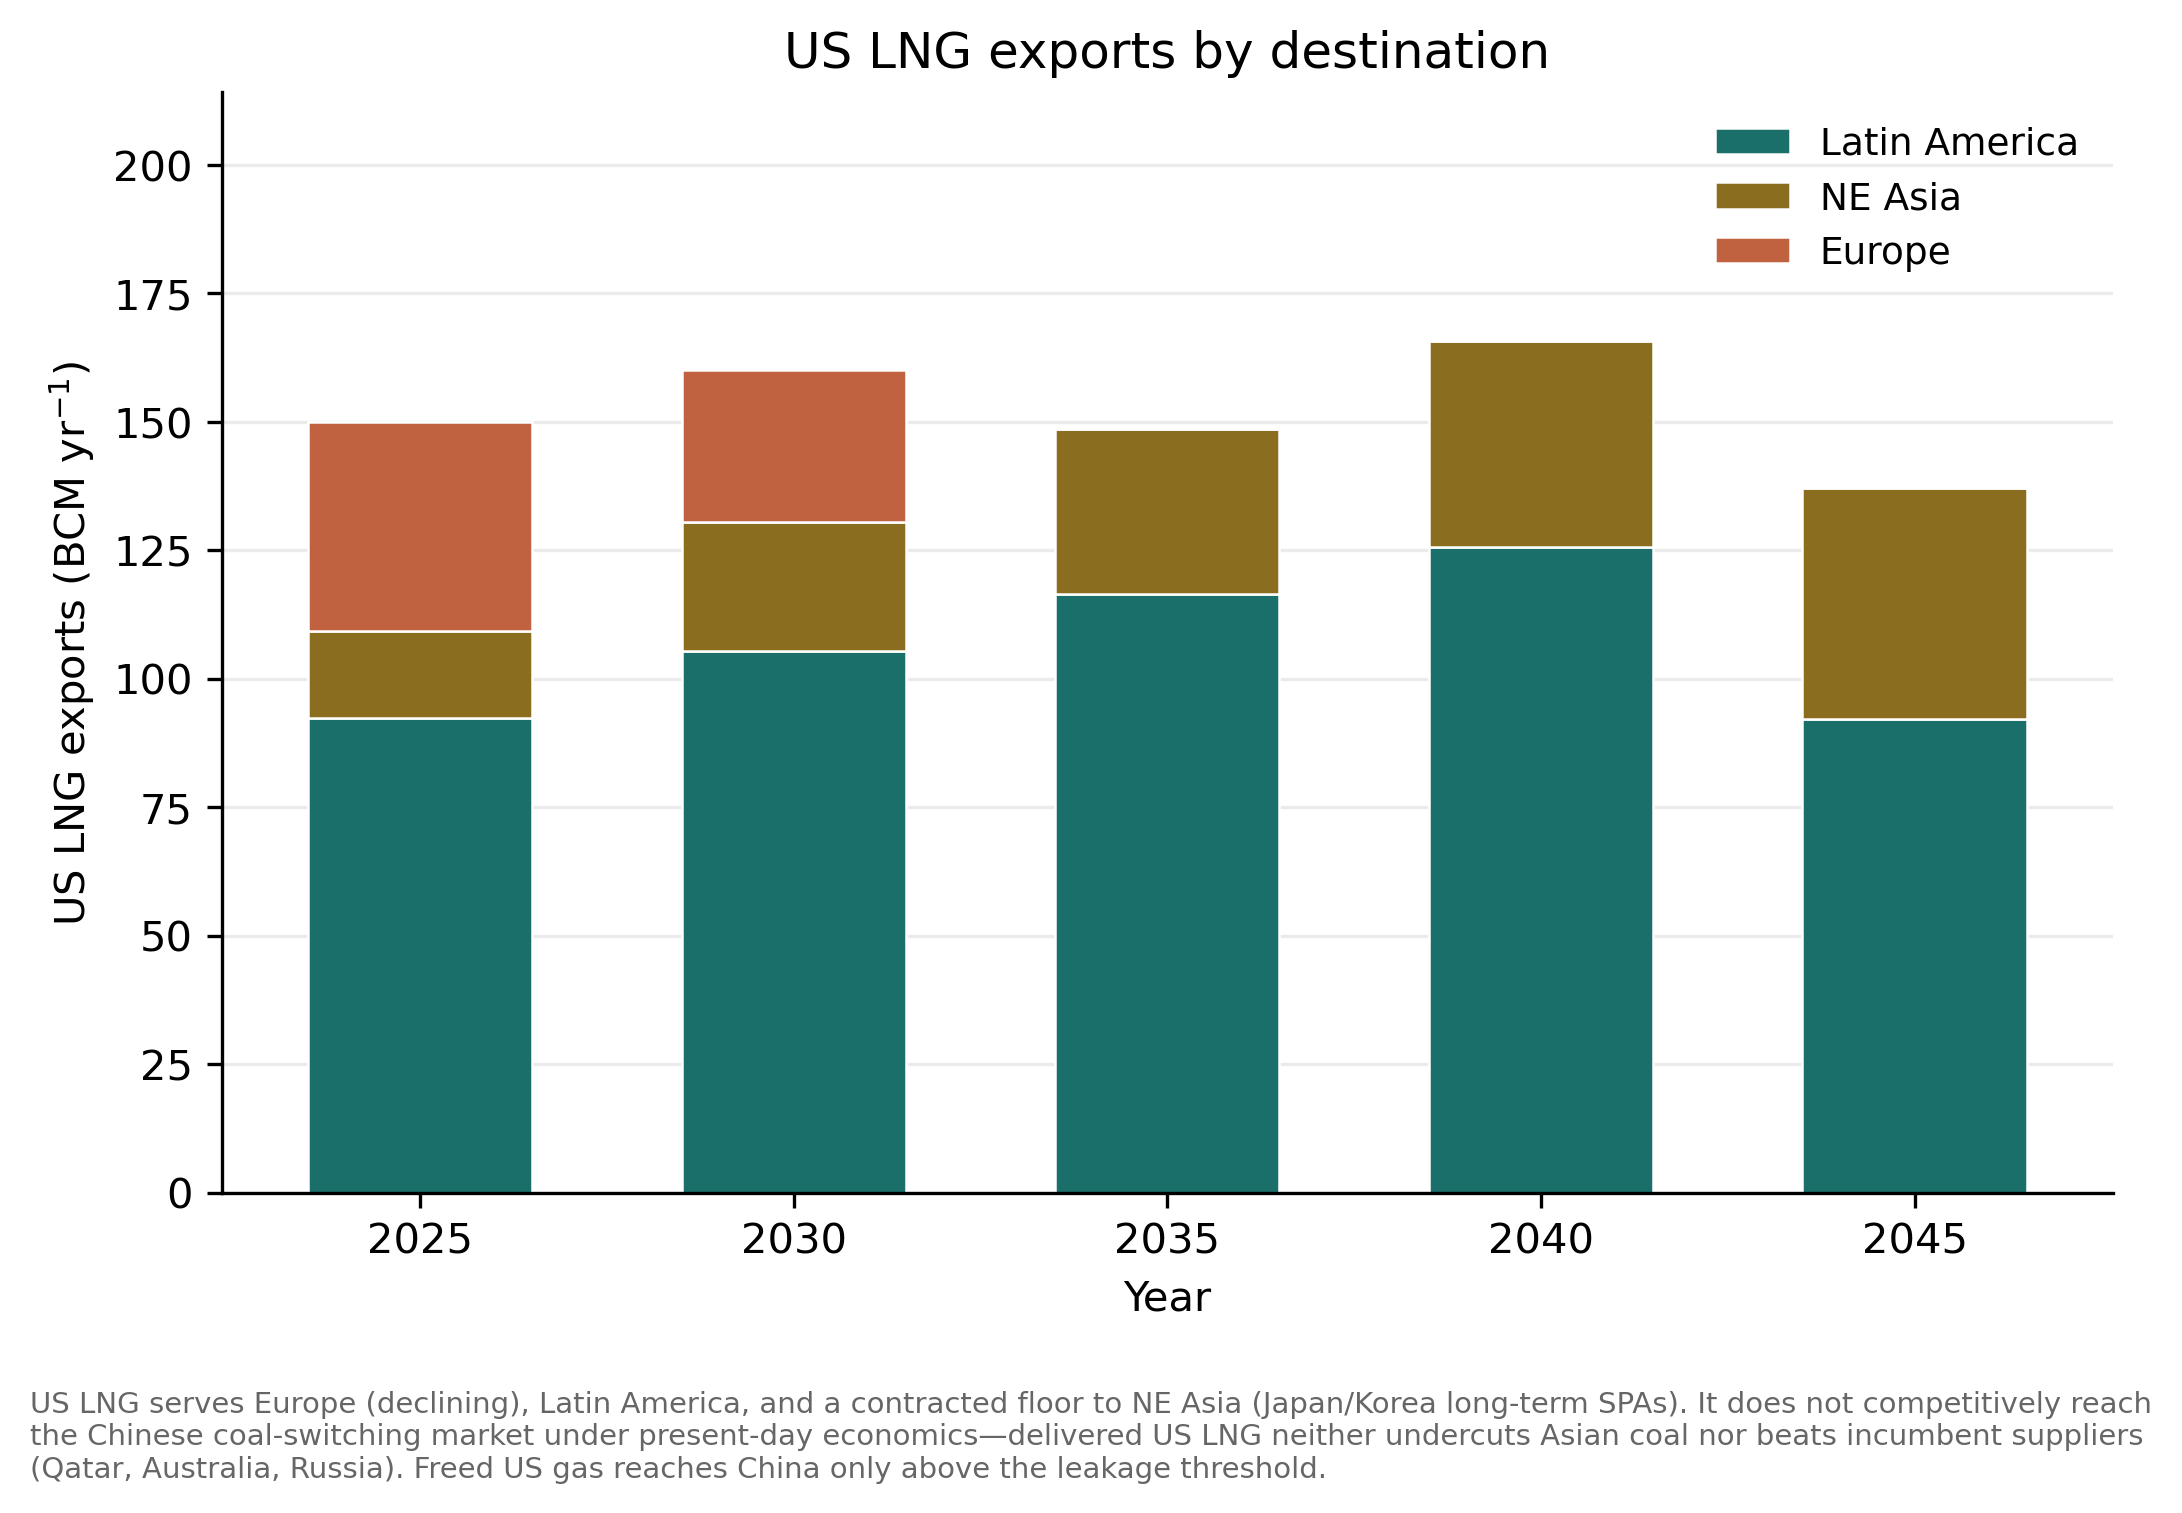
\includegraphics[width=0.9\linewidth]{outputs/figures/F5_us_lng_destinations.png}
\caption{Modelled US LNG exports by receiving market (BCM), 2025--2045. US LNG
serves Europe (declining as the post-2022 European LNG surge eases), Latin
America, and a contracted floor to NE Asia (Japan and South Korea, which hold
long-term US offtake contracts and were the fourth- and fifth-largest US LNG
destinations in 2023). It does \emph{not} competitively reach the Chinese
coal-switching market under present-day economics, because delivered US LNG
neither undercuts Asian coal nor beats the incumbent Asian suppliers (Qatar,
Australia, Russia) on delivered cost. This is the central ESL~$\approx$~0
result---freed US gas reaches the Chinese coal market and displaces coal only
once the reliability-premium or carbon-price threshold is
crossed.}\label{fig:lngdest}
\end{figure}

\begin{figure}[H]\centering
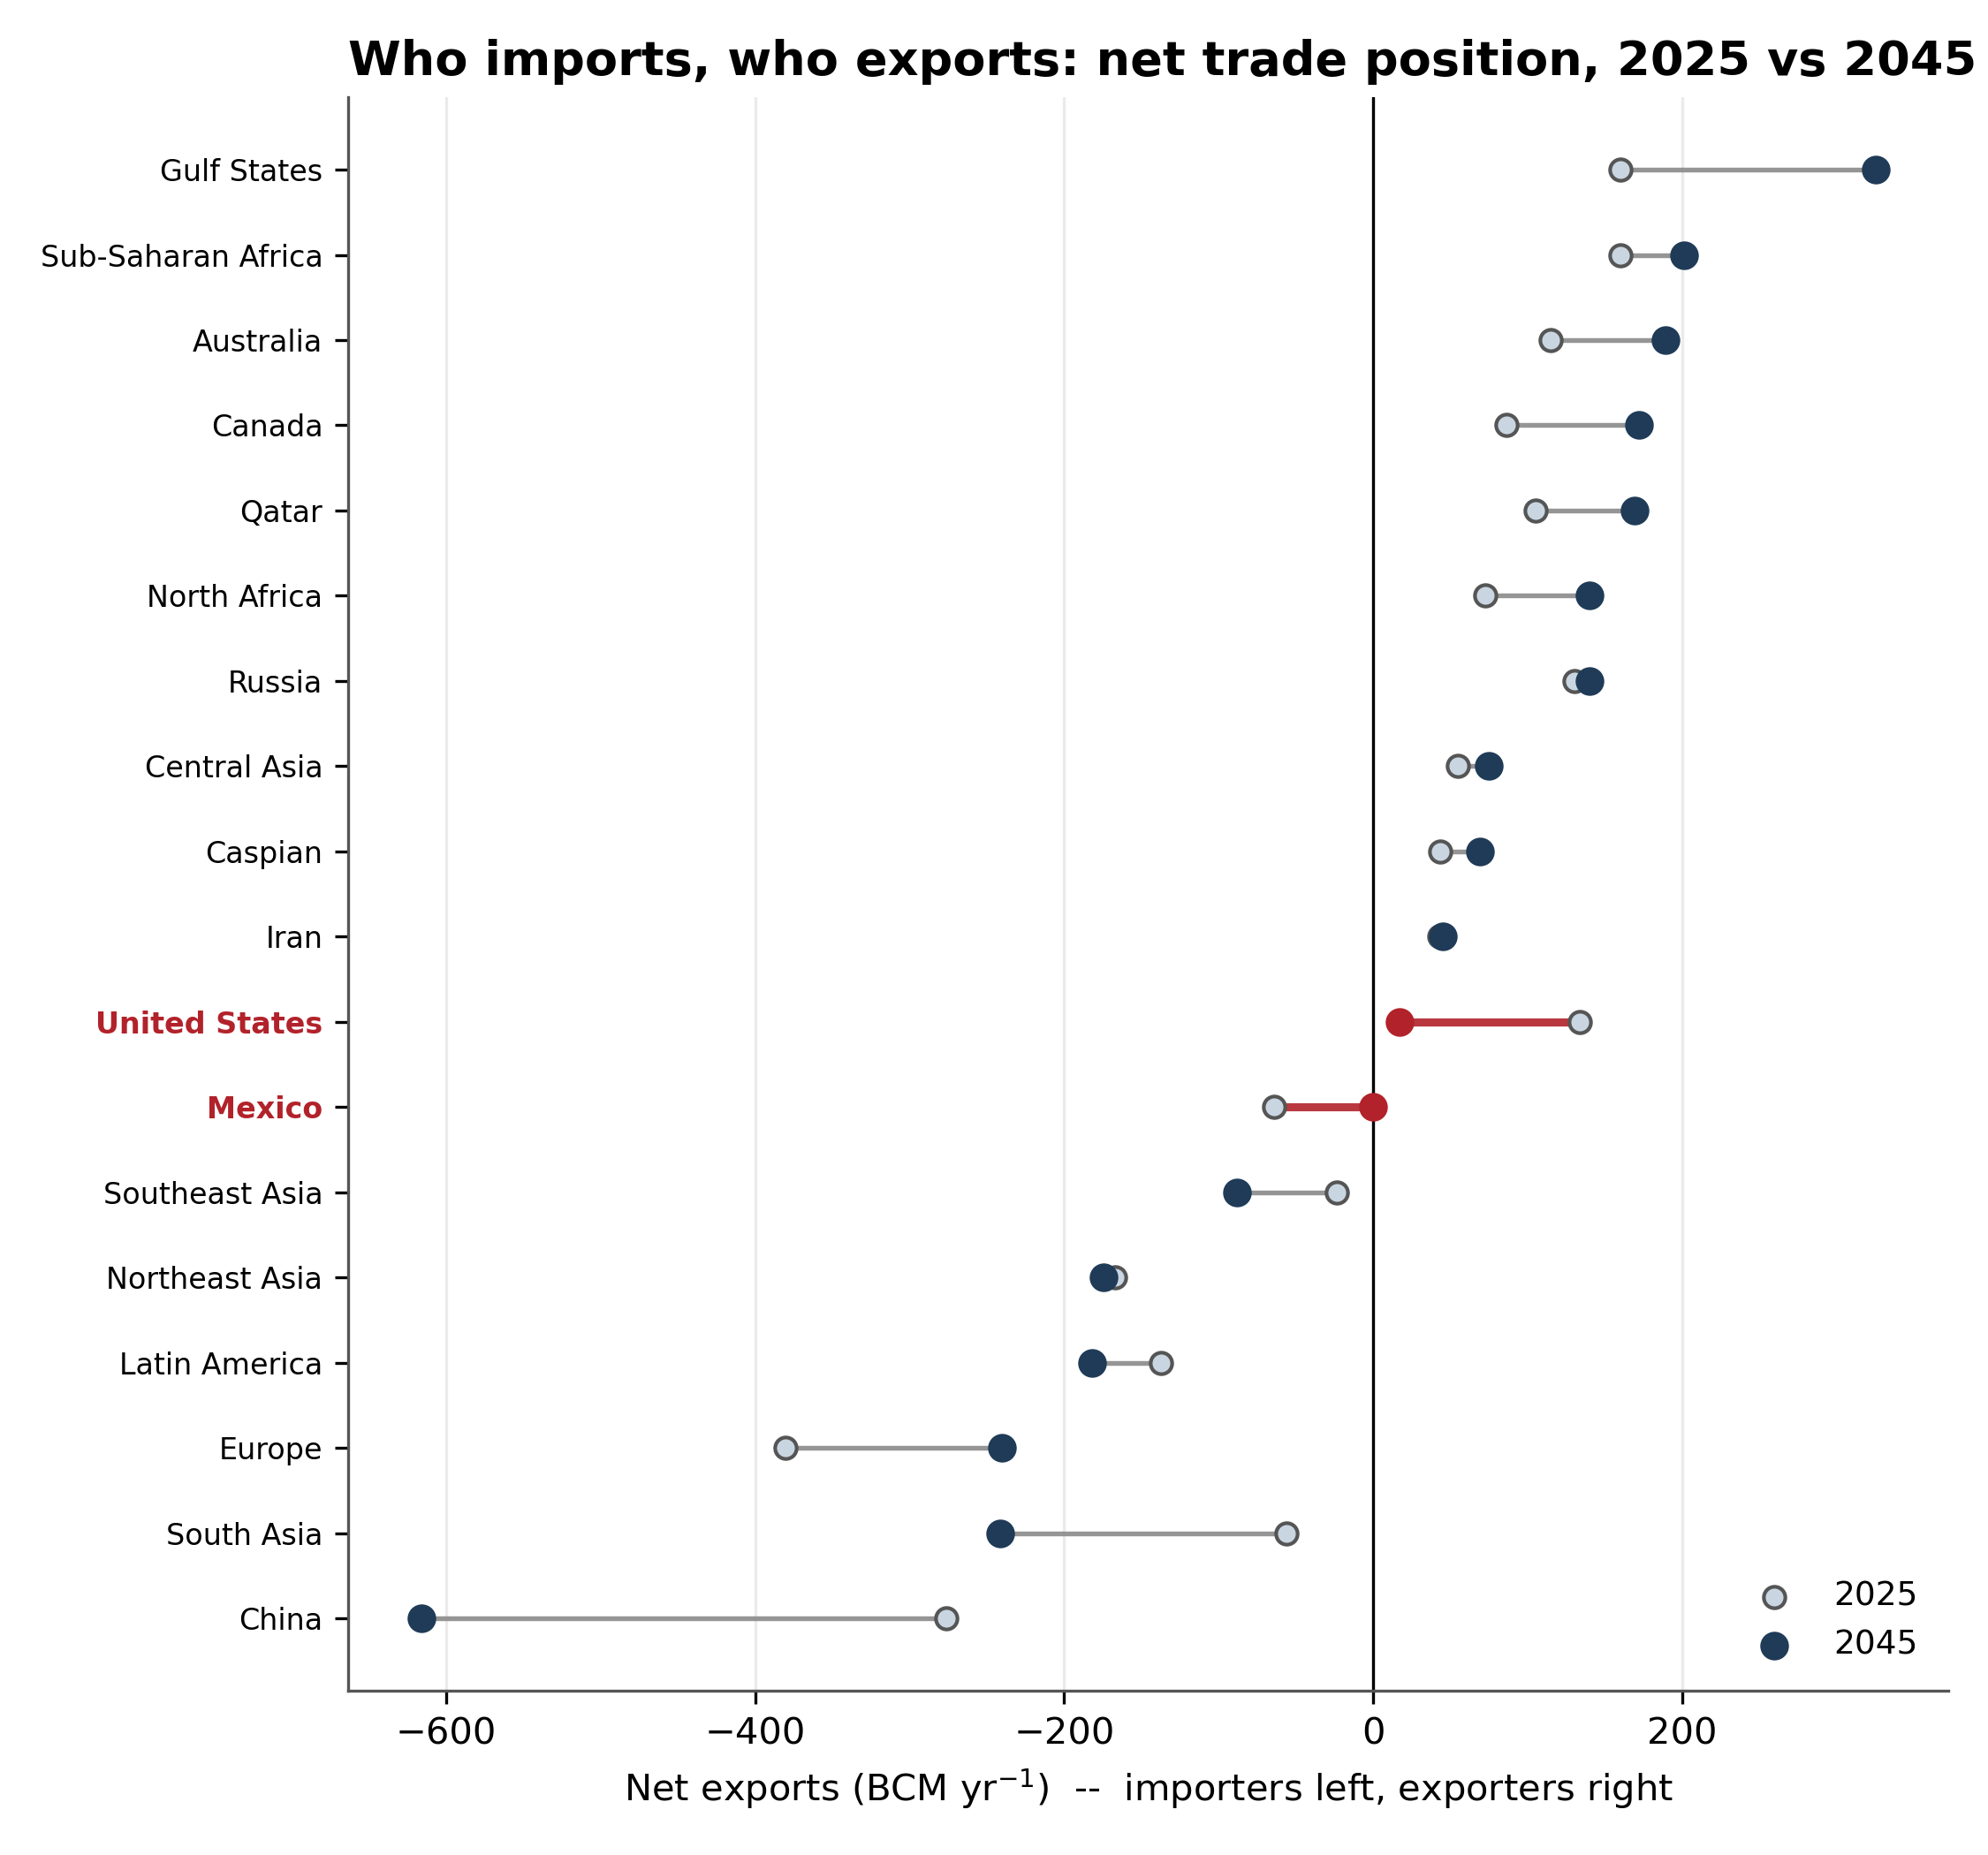
\includegraphics[width=0.85\linewidth]{outputs/figures/Region_net_trade_dumbbell.png}
\caption{Net trade position by region, 2025 versus 2045 (net exports:
production minus consumption; importers left of zero, exporters right).
Light points 2025, dark points 2045. Mexico (highlighted) moves from importer
toward self-sufficiency while the large Asian consumers deepen import
dependence---a repositioning of who produces and buys, not a reduction in
global gas use.}\label{fig:nettrade}
\end{figure}

\begin{figure}[H]\centering
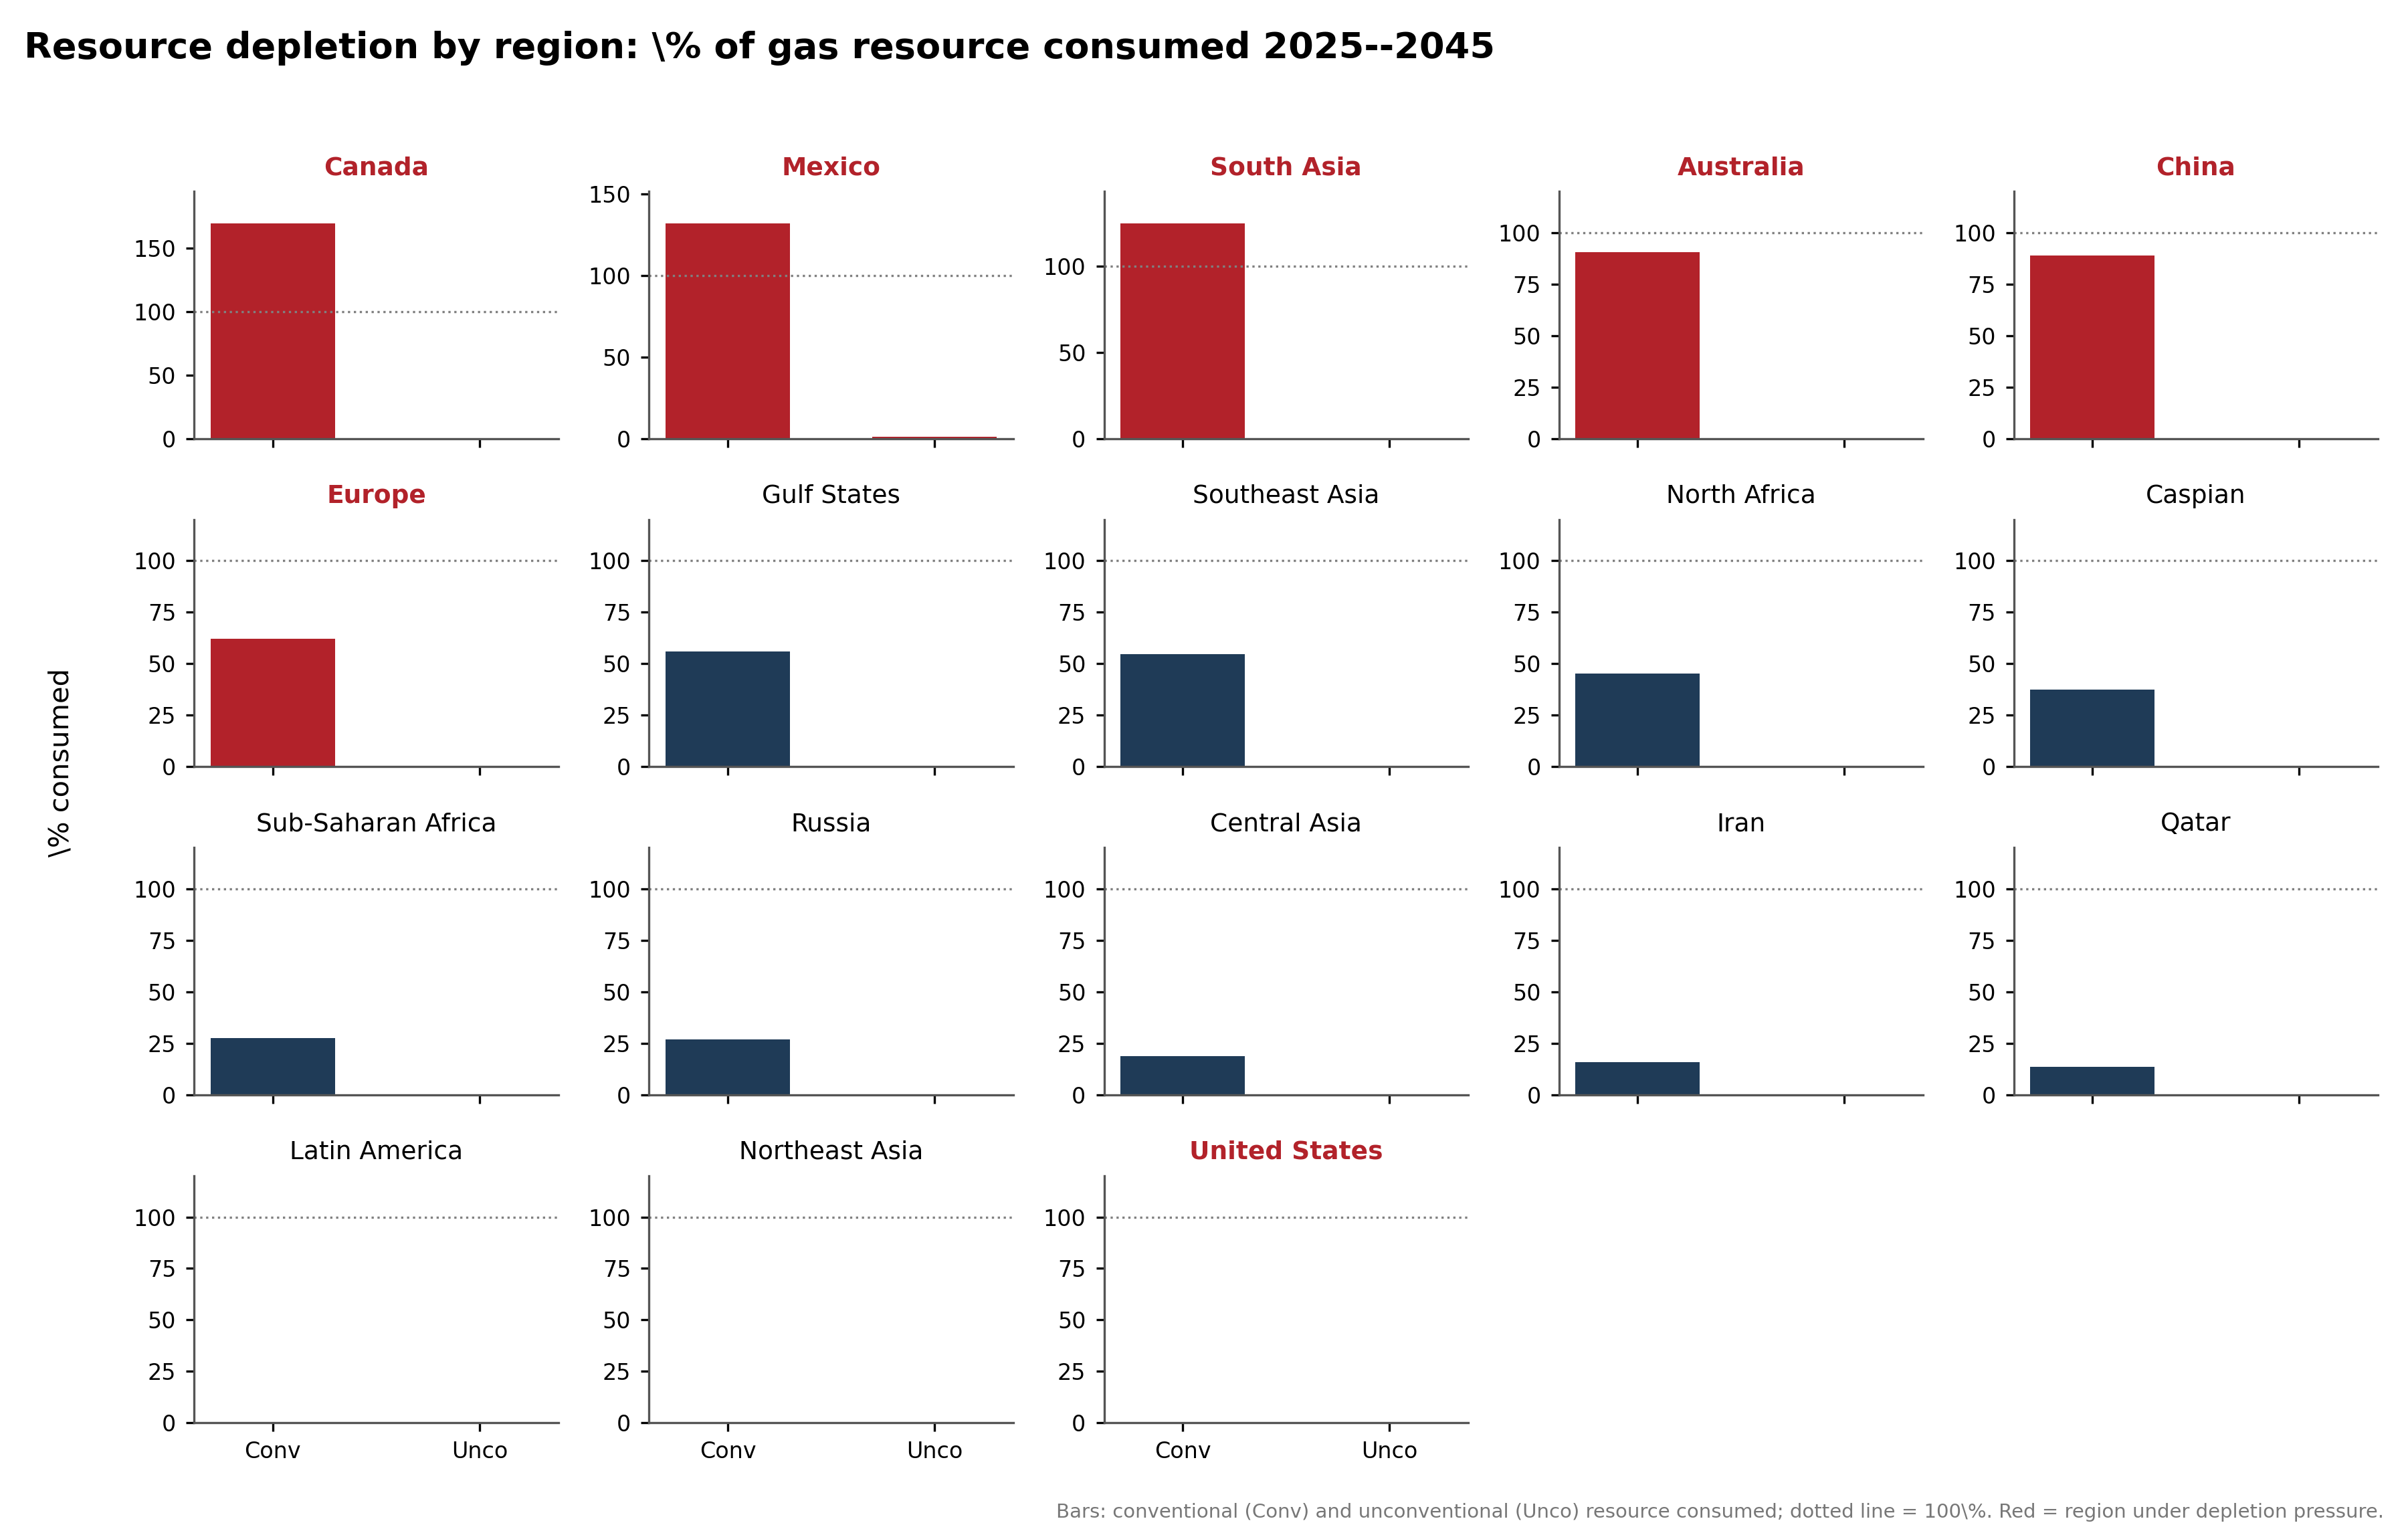
\includegraphics[width=\linewidth]{outputs/figures/Region_reserves_panels.png}
\caption{Resource depletion by region: percentage of each region's conventional
and unconventional gas resource base consumed over 2025--2045 under the
sovereignty case. Bars exceeding the dotted 100\% line indicate a resource base
outgrown by cumulative extraction (highlighted in red). Sustained re-export in
the leakage regime concentrates drawdown on the US unconventional base and a few
established exporters.}\label{fig:reserves}
\end{figure}

% ---------------------------------------------------------------
\section{Emissions accounting}\label{si:emissions}

The lifecycle intensities of the leaked molecule (US shale gas exported as LNG)
and of the coal it displaces are computed with a full ecoinvent 3.9.1
process-LCA \citep{Wernet2016} (IPCC~2021 characterisation, 1~MJ delivered;
\texttt{src/lca\_brightway.py}). The delivered-LNG pathway---extraction,
processing, liquefaction, trans-Pacific shipping and regasification---follows
supplier-specific LNG life-cycle inventories \citep{RomanWhite2021, Skone2019},
and the resulting import-chain intensity is consistent with independent
footprint assessments of gas delivered to Asia \citep{Gan2020}. At the central 2.5\% upstream methane rate the
leaked pathway is $\sim$90~gCO\textsubscript{2}e~MJ$^{-1}$
(GWP\textsubscript{100}) and $\sim$117 (GWP\textsubscript{20}), against
$\sim$108 and $\sim$126 for coal---so at central methane shale-LNG is
\emph{below} coal at both horizons and coal-to-gas switching is a net (if
modest) improvement. The sign reverses only at higher methane: shale-LNG and
coal break even at $\sim$3.1\% (GWP\textsubscript{20}) and $\sim$5.5\%
(GWP\textsubscript{100}) (Fig.~\ref{fig:methane}). The central rate and its 1.5--3.7\% range span the
values reported by aircraft, tower and satellite measurement campaigns, which
consistently exceed bottom-up inventories and vary strongly by basin
\citep{Alvarez2012, Brandt2014, Schwietzke2016, Zhang2020, Lauvaux2022}; this
measurement--inventory gap is exactly why we treat the climate sign as
methane-contingent. Emissions are attributed at the margin (leaked gas
burned minus coal displaced); model intensity units convert to mass with
$1~\mathrm{BCM} \approx 36$~PJ, i.e. $0.036$~Mt~CO\textsubscript{2}e per unit.

\begin{figure}[H]\centering
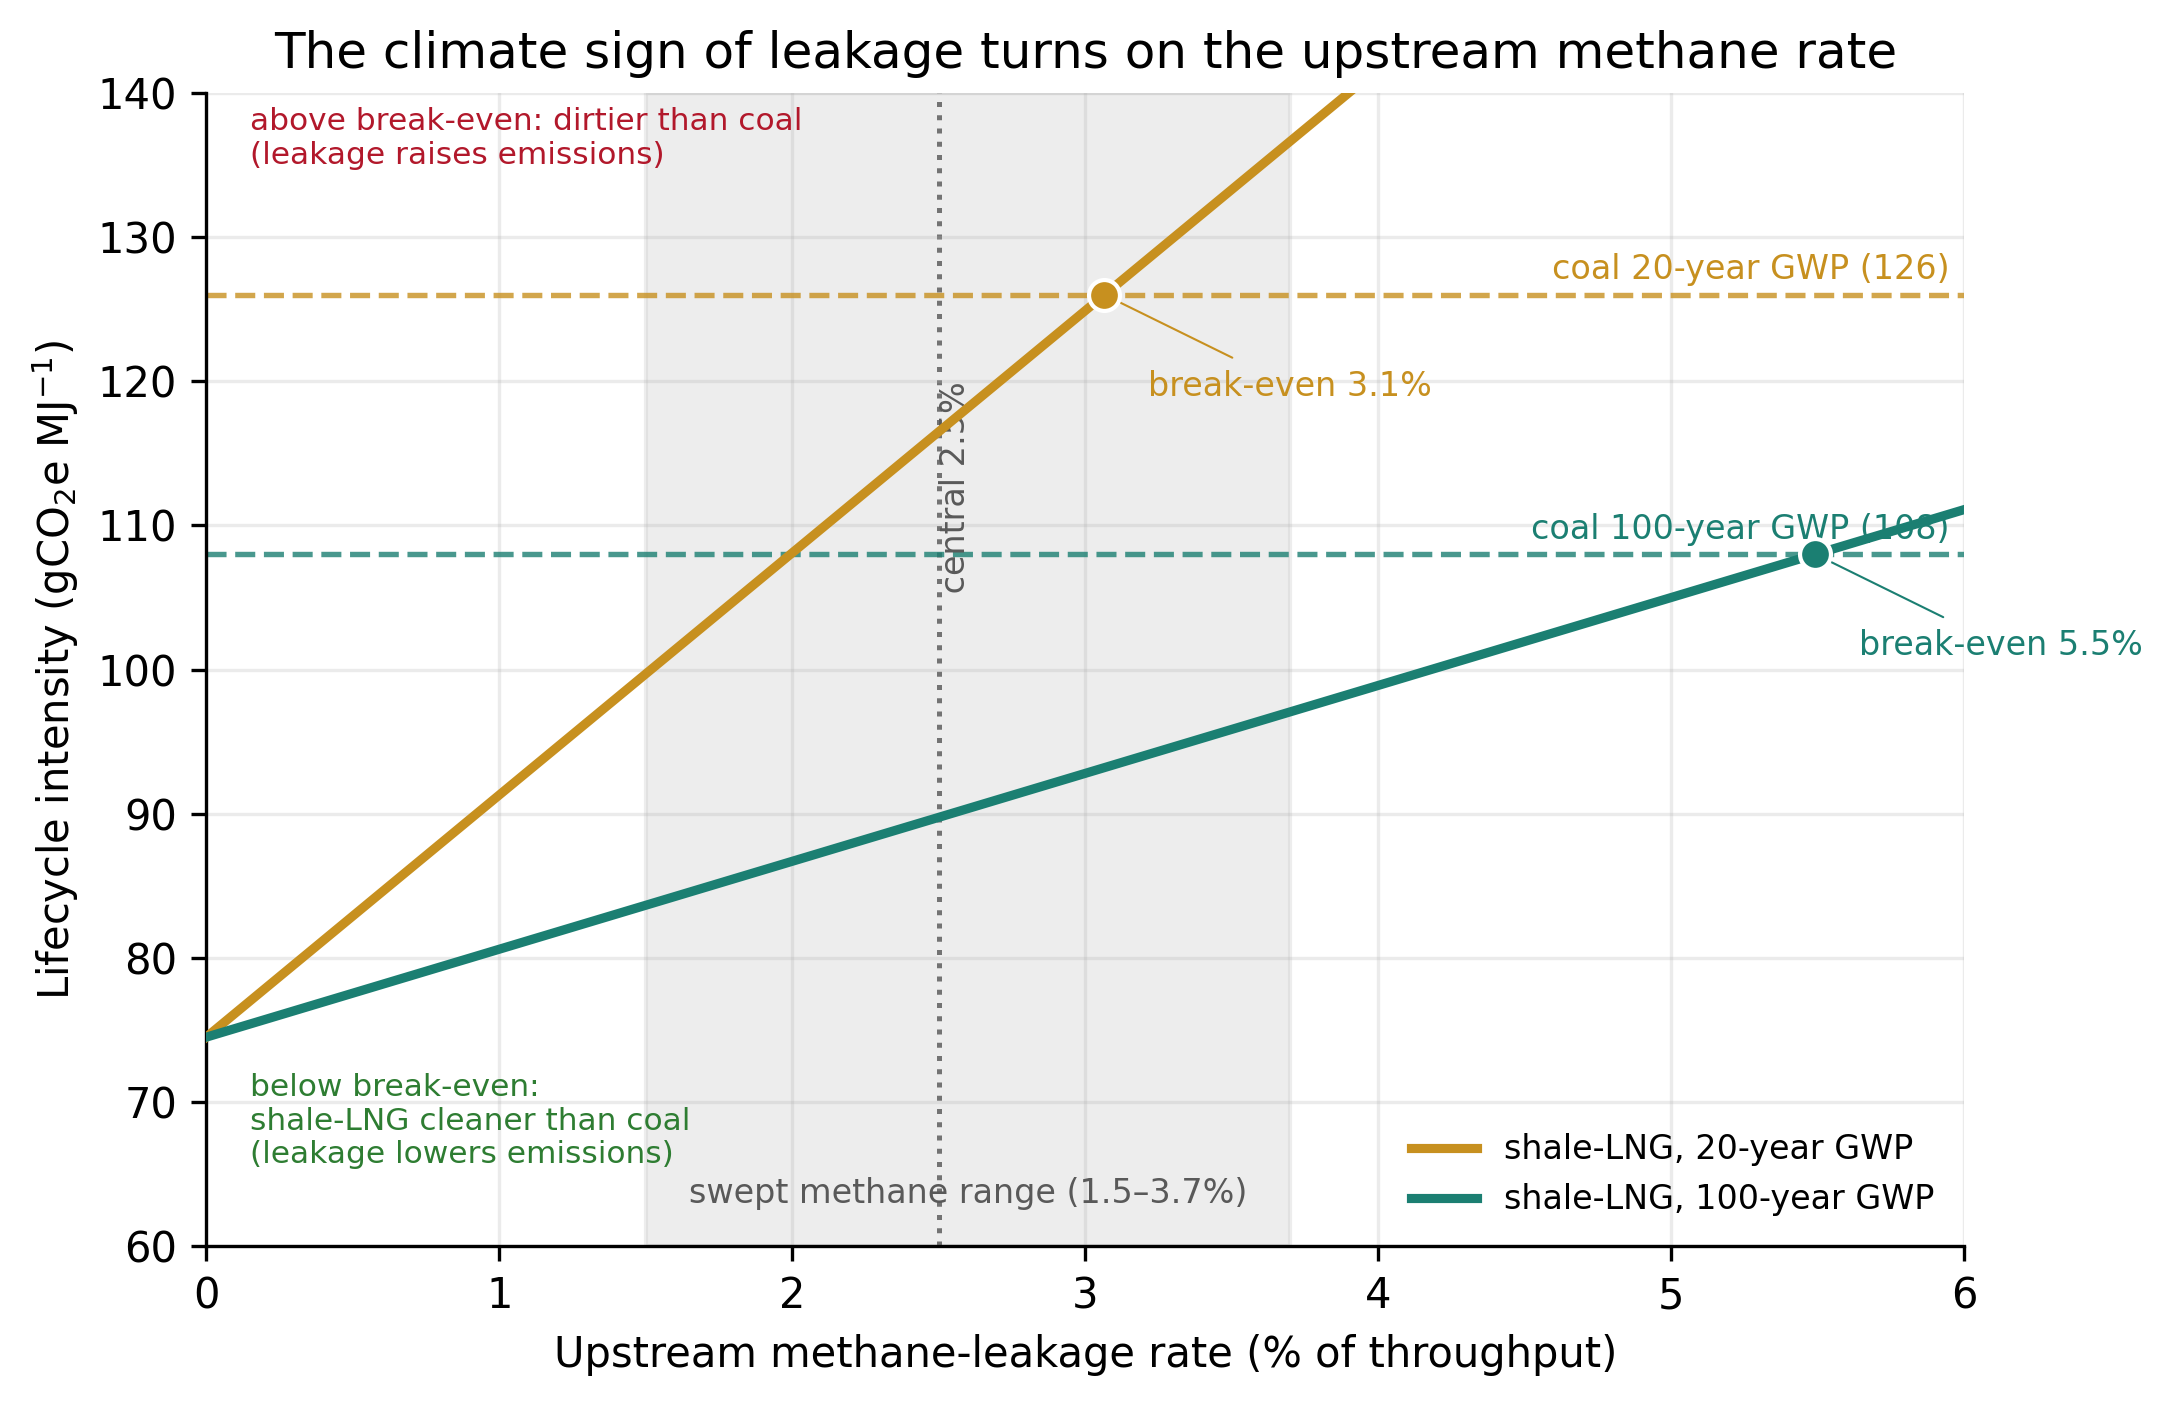
\includegraphics[width=0.82\linewidth]{outputs/figures/Methane_contingency.png}
\caption{The climate sign of leakage turns on the upstream methane rate.
Delivered shale-LNG lifecycle intensity $I_{\mathrm{gas}}=a+b\,r$ (methane-%
independent part $a=74.5$; per-percent methane term $b=6.1$ on a 100-year and
$16.8$ on a 20-year GWP) as a function of the upstream methane-leakage rate $r$,
against the fixed intensity of the Asian coal it displaces (dashed). The swept
methane range (1.5--3.7\%) is shaded and the central 2.5\% rate marked. Shale-LNG
crosses coal---so leakage flips from lowering to raising emissions---at
$r\approx3.1\%$ on the 20-year horizon (inside the swept range) and
$r\approx5.5\%$ on the 100-year horizon. At the central rate shale-LNG is below
coal at both horizons; the ranking, and hence the climate sign of ESL, reverses
within the measurement-supported methane range on the near-term
horizon.}\label{fig:methane}
\end{figure}

\paragraph{Note on an earlier methane basis.} An initial parametric ledger
expressed upstream methane as $E_{\mathrm{comb}}\,(r/100)\,\mathrm{GWP}$, using
the combustion CO\textsubscript{2} intensity ($E_{\mathrm{comb}}=56$) as the
base. This overstates the methane term by the CO\textsubscript{2}/CH\textsubscript{4}
mass ratio ($44/16\approx2.75$): the leaked mass scales with CH\textsubscript{4}
\emph{throughput} ($\sim$20.4~g~CH\textsubscript{4}~MJ$^{-1}$), not with the CO\textsubscript{2}
produced when it burns. Correcting this (and adopting the ecoinvent coal
intensity, which includes coal-mine methane, a large and growing source in its
own right \citep{Kholod2020}) moves the central result from
``shale-LNG above coal at both horizons'' to ``shale-LNG below coal at 2.5\%
methane, above only for methane $>\sim$3\% under GWP\textsubscript{20}''. The
ecoinvent process-LCA independently confirms the corrected values.

The stage decomposition (Fig.~\ref{fig:lca}) resolves the gas pathway into
extraction and processing, upstream methane, liquefaction, shipping, and
combustion, and coal into mining plus coal-mine methane, transport, and
combustion, reproducing the ecoinvent totals (gas 90/117, coal 108/126
gCO\textsubscript{2}e~MJ\textsuperscript{-1} at
GWP\textsubscript{100}/GWP\textsubscript{20}). It makes plain that the outcome
turns on \emph{upstream methane}: at 2.5\% the methane segment is not large
enough to lift shale-LNG above coal, but it grows steeply with the leak rate
and dominates the comparison at the 20-year horizon.

\begin{figure}[H]\centering
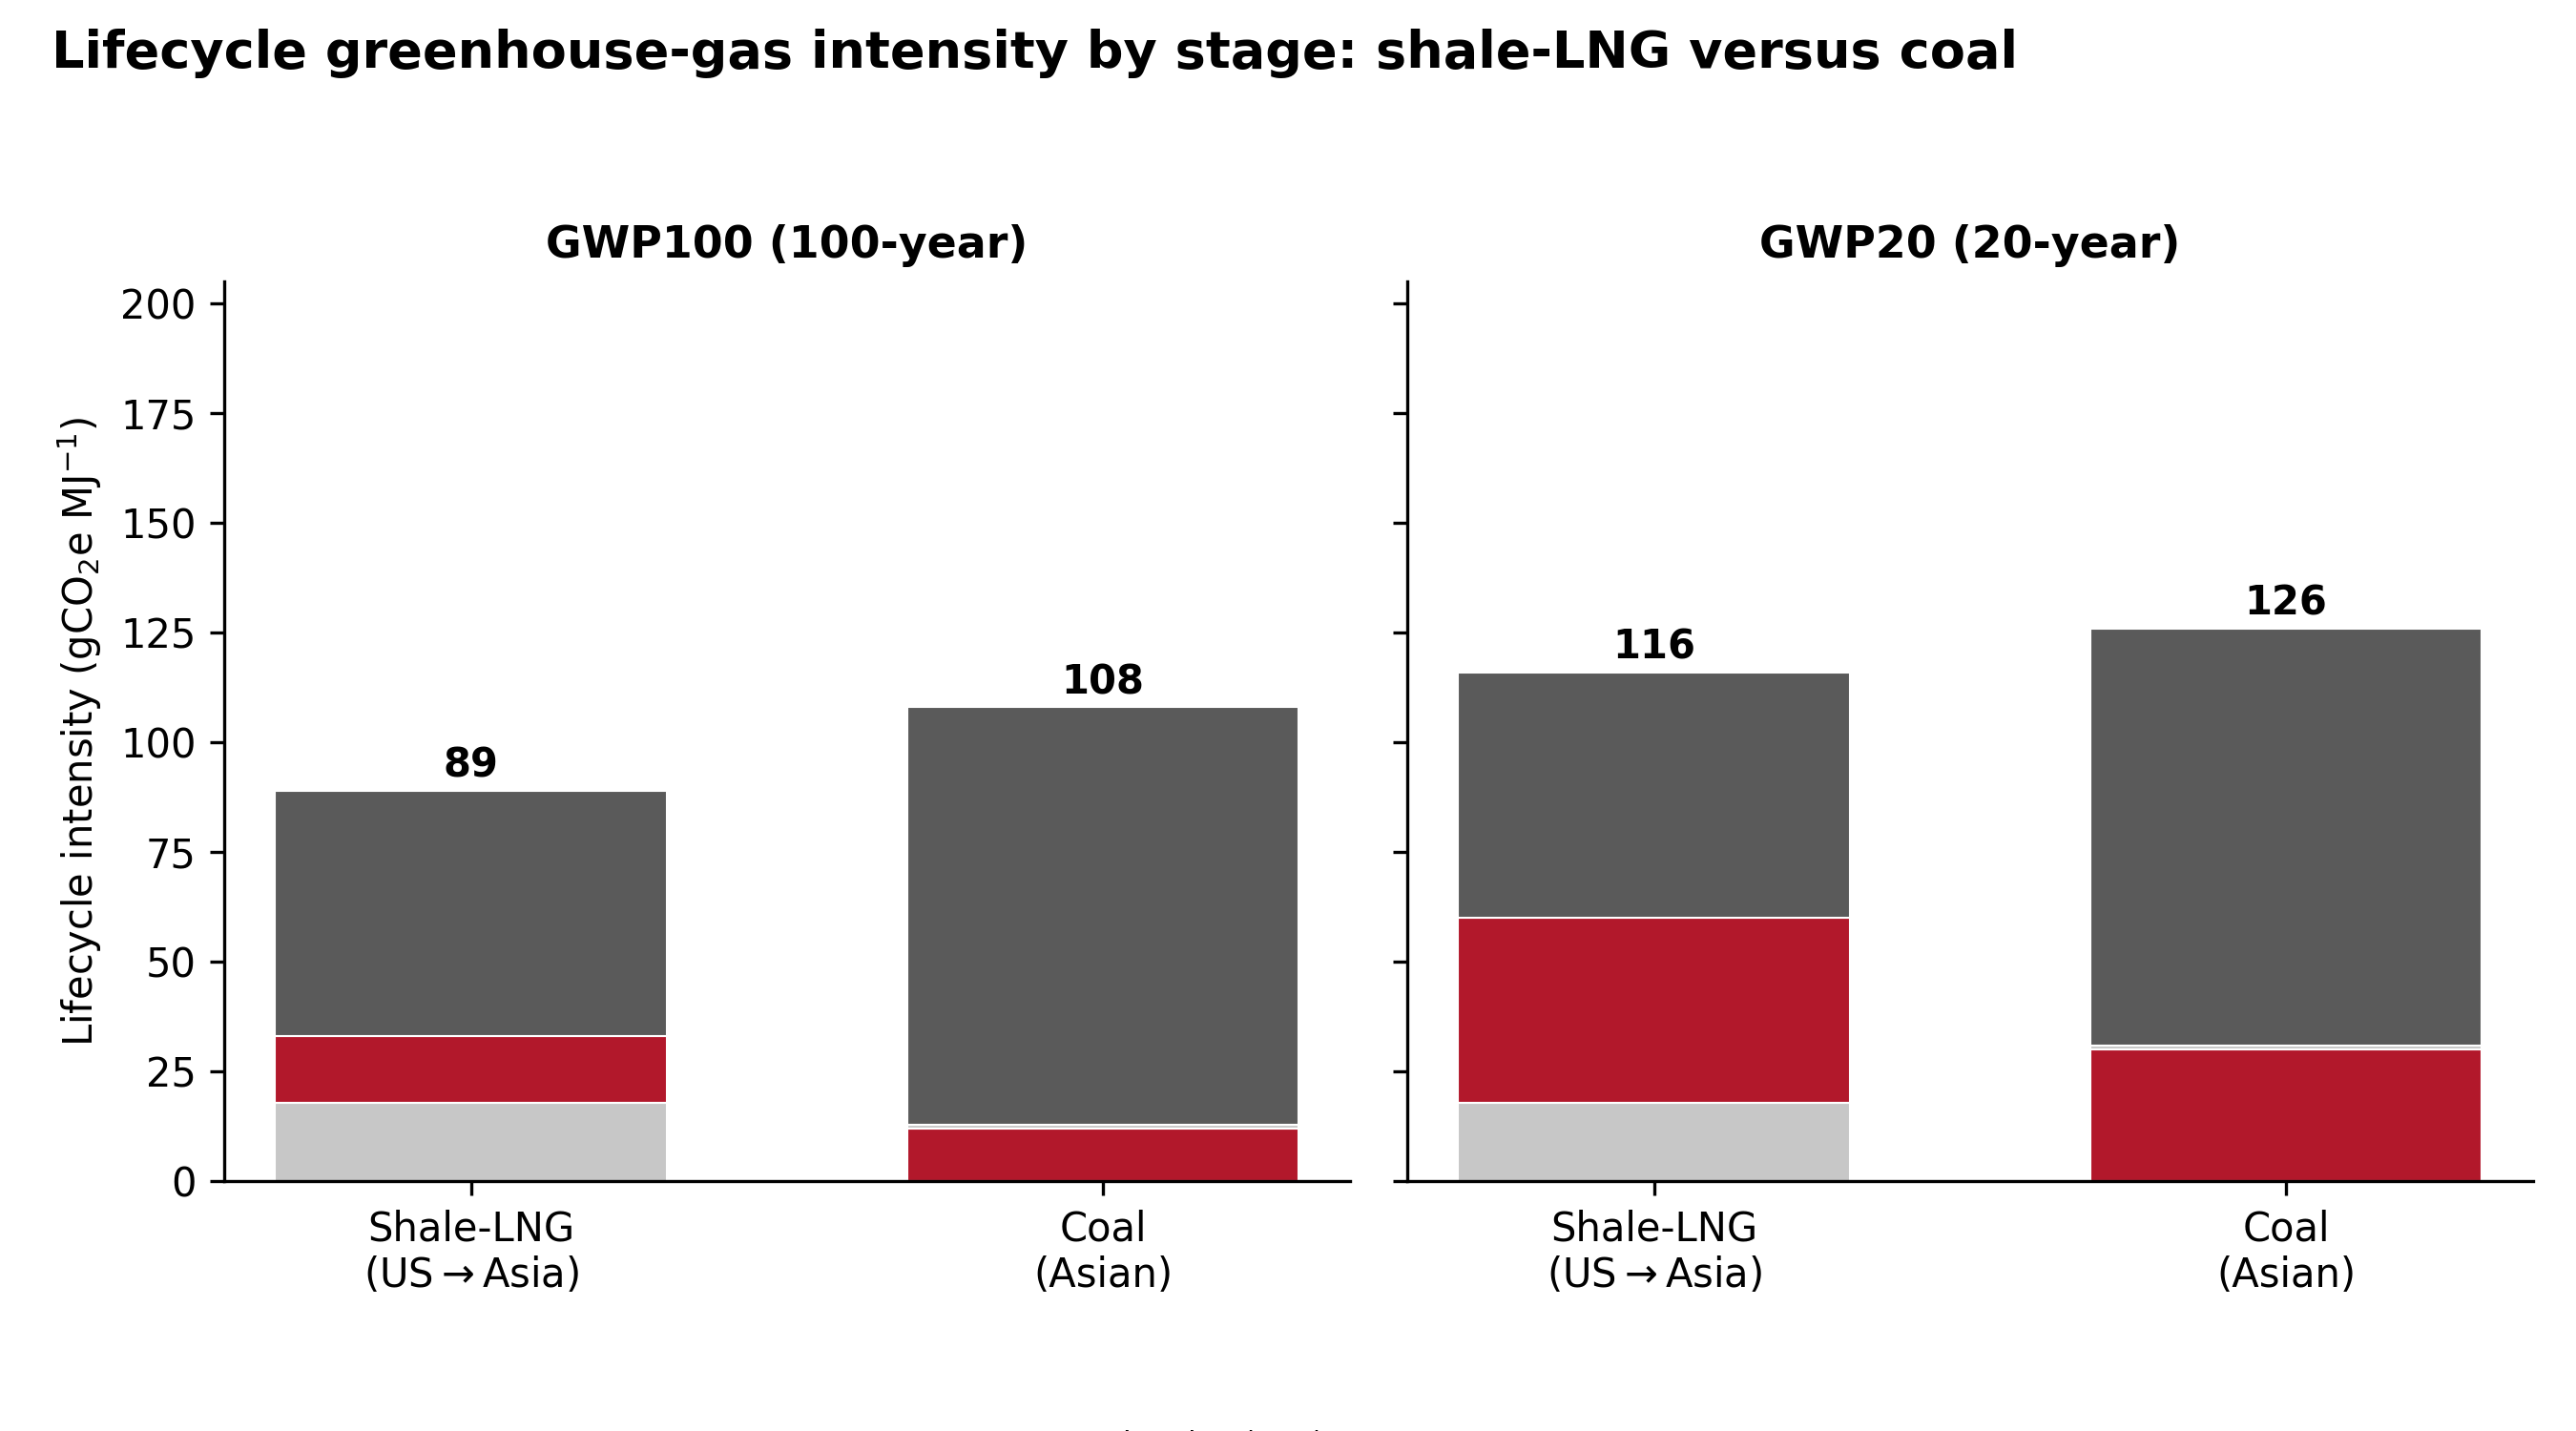
\includegraphics[width=0.9\linewidth]{outputs/figures/LCA_stage_decomposition.png}
\caption{Stage-resolved lifecycle greenhouse-gas intensity of US shale gas
delivered to Asia as LNG versus the Asian coal it displaces, under 100-year
(left) and 20-year (right) GWP, at 2.5\% upstream methane. Bar totals equal the
intensities used in the emissions ledger (gas 90/117, coal 108/126); the red
segment is upstream/mine methane. At this methane rate shale-LNG sits below
coal at both horizons; the methane segment---and hence the ranking---rises with
the leak rate.}\label{fig:lca}
\end{figure}

\subsection{The PyPSA\,$\times$\,Brightway coupling in detail}\label{si:coupling}

Emissions are not accounted for by a fixed emission factor but by coupling the
trade optimisation directly to a process-lifecycle inventory. This subsection
sets out the coupling in full, since it is, to our knowledge, one of the first
global energy-system trade models linked to a complete process-LCA at every
iteration. The overall methodology and the coupling are summarised by the methodology
flowchart (Extended Data Fig.~1); Listing~\ref{lst:coupling} gives the coupling
as pseudocode.

\paragraph{Why a coupling, and why it is exact.} A life-cycle impact score is a
linear functional of the inventory: doubling an activity's functional-unit
amount doubles its characterised impact. Consequently the characterised
intensity of an activity---greenhouse-gas emissions per megajoule of delivered
gas, say---can be evaluated \emph{once} in Brightway and then multiplied by the
activity level chosen by the optimiser, for any dispatch, without re-running the
LCA. This is what makes an ``every-iteration'' coupling tractable: the
expensive step (building and characterising the inventory) is done once per
calibration, and each solved year is mapped to emissions by a matrix--vector
product. The alternative---re-solving a full LCA inside every optimisation
iteration---would be prohibitively slow and, because of linearity, would give
identical results.

\paragraph{Inventory.} Lifecycle intensities are built on a licensed ecoinvent
3.9.1 background in Brightway (\texttt{src/lca\_brightway.py}), characterised
with the IPCC~2021 method at both GWP\textsubscript{100} and GWP\textsubscript{20}
and a functional unit of 1~MJ of delivered gas (respectively 1~MJ of coal). The
gas supply chain (extraction, processing, liquefaction, shipping and
regasification) is taken from the ecoinvent US LNG import chain; coal from the
hard-coal mine, preparation and rail-transport activities. Combustion
CO\textsubscript{2} is added explicitly (56.1~gCO\textsubscript{2}~MJ$^{-1}$ for
gas). One structural feature of ecoinvent 3.9.1 is important: it contains no
shale-specific gas activity and no per-country ``natural gas, high pressure''
production process (gas is a co-product of petroleum production). Its built-in
upstream methane is therefore a database average of order 1\%. Because the
central question of this paper is the effect of the \emph{higher},
measurement-based US-shale methane rate, we do not rely on the database value:
we take the methane-independent lifecycle intensity from ecoinvent
($a=74.5$~gCO\textsubscript{2}e~MJ$^{-1}$, combustion plus non-methane
upstream/LNG-chain CO\textsubscript{2}, identical at both horizons because it is
CO\textsubscript{2}) and add upstream methane explicitly at the swept rate,
on the CH\textsubscript{4}-throughput basis,
\begin{equation}
I_{\mathrm{gas}}^{(h)}(r) = a + b^{(h)}\, r, \qquad
b = \{6.1,\,16.8\}\ \mathrm{gCO_2e\,MJ^{-1}\,per\ \%},
\end{equation}
so that per-resource-type methane rates from \texttt{data/technology.csv}
(shale 2.5\%, mature/dry shale 0.6\%, offshore 0.4\%, conventional 1.0\%) give
distinct intensities for each supply type. This makes the resource-type methane
assumption an explicit, auditable model input rather than a hidden database
default---and it is exactly the parameter on which the climate result turns.

\paragraph{From dispatch to per-region emissions.} For each solved year the
coupling (\texttt{src/lca\_link.py}) assembles each region's lifecycle
emissions, without double counting, as
\begin{equation}
E_{\mathrm{region}} = \sum_{\mathrm{prod}} p_g\,I^{\mathrm{up}}_{\mathrm{tech}(g)}
 \;+\; D\,I_{\mathrm{comb}} \;+\; X_{\mathrm{LNG}}\,I_{\mathrm{LNG}}
 \;+\; C_{\mathrm{coal}}\,I_{\mathrm{coal}},
\end{equation}
i.e. the upstream (cradle-to-gate) emissions of what the region \emph{produces}
by resource type, the combustion of what it \emph{consumes}, the LNG-chain
emissions of what it \emph{exports} as LNG, and the coal it still burns where
gas does not displace it. Volumes convert from BCM to mass with
$1~\mathrm{BCM}\approx36$~PJ. The coupling therefore returns per-region,
per-year lifecycle emissions at both horizons (shown in the main text),
consistent by construction with the
marginal ledger used for the ESL climate result: the same intensities that
decide the marginal shale-LNG-versus-coal comparison also drive the system-wide,
per-region totals. Listing~\ref{lst:coupling} states the procedure.

\begin{lstlisting}[style=coupling, caption={The PyPSA\,$\times$\,Brightway
coupling, in pseudocode. The Brightway inventory is characterised once (lines
2--7); each solved year of the trade optimisation is mapped to per-region
lifecycle emissions by a linear application of those intensities to the
dispatch (lines 9--21).}, label={lst:coupling}]
# ---- ONCE per calibration: lifecycle intensities from Brightway ----
setup_project(ecoinvent="3.9.1", method="IPCC 2021")   # GWP100 & GWP20
I_comb  = 56.1                                    # gCO2e/MJ, gas combustion
I_lng   = lcia("US LNG chain")                    # non-CH4 upstream + liquefaction/ship/regas
I_coal  = lcia("hard coal, mine+transport+comb")  # {108, 126} gCO2e/MJ
for tech in gas_technologies:                     # explicit upstream methane,
    I_up[tech] = a_nonCH4 + b * CH4_rate[tech]     #   by resource type (a=74.5, b={6.1,16.8})

# ---- EVERY solved year of the optimisation ----
for year in YEARS:
    n = build_network(year)
    apply_scenario(n, scenario, premium=rho, carbon_price=tau)
    n.optimize()                                  # convex QP -> dispatch p_g, flows f_l
    for region in regions:
        E[region, year] = (
              sum(p_g * I_up[tech(g)] for g in producers[region])   # upstream
            + demand[region]        * I_comb                        # combustion
            + lng_exports[region]   * I_lng                         # LNG chain
            + coal_burned[region]   * I_coal )                      # residual coal
        # (converted BCM -> Mt with 1 BCM ~ 36 PJ)
return E     # per-region, per-year lifecycle emissions at both GWP horizons
\end{lstlisting}

\paragraph{Scope and limitations.} The coupling is attributional at the process
level and consequential only through the optimiser's dispatch response; it does
not endogenise capital-stock lifecycle emissions (pipelines, terminals) or
demand-side rebound beyond the coal-switching channel. Its dominant uncertainty
is the upstream methane rate, which we therefore sweep rather than fix. The
ecoinvent background could be updated to a prospective database (e.g. via
scenario-consistent electricity mixes) without changing the coupling
architecture.

% ---------------------------------------------------------------
\section{Data and code availability}\label{si:data}

All input data derive from public sources: the Energy Institute Statistical
Review of World Energy \citep{EI2024}, US EIA, IEA \citep{iea_methane_2024},
and the EIA/ARI world shale assessment \citep{EIA_ARI2013}. Model code
(PyPSA), scenario definitions, the ESL and threshold drivers, and all
plotting scripts are available at
\texttt{https://github.com/kerdan85/GlobalGasModel} and archived at
\texttt{https://doi.org/10.5281/zenodo.24039785}. Calibration sources
and assumptions are documented in \texttt{CALIBRATION\_NOTES.md}.

\bibliographystyle{plainnat}
\bibliography{sn-bibliography}

\end{document}
